% ------------------------------------------------------------------------
%
% -------------------      Plantilla_UIS.tex       -----------------------
%
% ------------------------------------------------------------------------
% ------------------------------------------------------------------------
% ------------------------------------------------------------------------
% Versión de plantilla para realización de informes de trabajo de grado
% construida para uso de la Universidad Industrial de Santander.
%
% Reservados todos los derechos
%
% Bucaramanga, Colombia
%
% Septiembre 17 de 2018
%
% ------------------------------------------------------------------------
% ------------------------------------------------------------------------
% ------------------------------------------------------------------------
%
% ------------------------------------------------------------------------
\documentclass[letter,oneside,12pt,spanish]{report}          % Encabezados
\usepackage[utf8]{inputenc}
%\usepackage[latin]{babel}
% ------------------------------------------------------------------------
\usepackage{icontec_style}                   % Libreria UIS ICONTEC
% ------------------------------------------------------------------------
% Ingrese en este punto las librerías específicas de usuario
% ------------------------------------------------------------------------
\usepackage{amsmath}
\usepackage{amssymb}
\usepackage{subfigure}
\usepackage{hyperref}
\usepackage{float}
\usepackage{graphicx}
\usepackage{algorithm,algpseudocode}
\usepackage{xcolor}
\setcounter{tocdepth}{4} % show also subsections in toc
\setcounter{secnumdepth}{4} % show also subsections number in toc
% ------------------------------------------------------------------------
% Archivo de bibliografía
% ------------------------------------------------------------------------
\addbibresource{references.bib}
% ------------------------------------------------------------------------
\def\autor{David Santiago Morales Norato}
\def\titulo{Algoritmo de clasificación de objetos en imágenes difractivas basado en medidas cuadráticas codificadas usando un enfoque de aprendizaje profundo}
\def\director{Andrés Felipe Jerez Ariza}
\def\codirector{Henry Arguello Fuentes}
\def\universidad{Universidad Industrial de Santander}
\def\escuela{Escuela de Ingeniería de Sistemas e Informática}
\def\facultad{Facultad de Ingenierías Fisicomecánicas}
\def\grupo{Grupo de Investigación en Diseño de Algoritmos y Procesamiento de Datos Multidimensionales (HDSP)}
\def\fecha{2022}
\def\codigo{2170102}

\DeclareMathOperator*{\minimize}{minimizar} % Declaración operador minimize

\DeclareMathOperator*{\maximize}{maximizar} % Declaración operador maximize
\DeclareMathOperator*{\subjectto}{sujeto \ a} % Declaración operador subjectto
\DeclareMathOperator*{\argmax}{arg \ max} % Declaración operador arg max

\DeclareMathOperator*{\argmin}{arg \ min} % Declaración operador arg min

\DeclareMathOperator*{\min}{min} % Declaración operador arg min

\newtheorem{definition}{Definición}% Declaración segmento definición matemática


% Traducción de palabras reservadas del algoritmo a español
\newenvironment{algoritmo}[1][]
  {\begin{algorithm}[#1]
     \selectlanguage{spanish}%
     \floatname{algorithm}{Algoritmo}%
     \renewcommand{\algorithmicif}{\textbf{si}}%
     \renewcommand{\algorithmicthen}{\textbf{entonces}}%
     \renewcommand{\algorithmicend}{\textbf{fin}}%
     \renewcommand{\algorithmicfor}{\textbf{para}}%
     \renewcommand{\algorithmicdo}{\textbf{hacer}}%
     % Set other language requirements
  }
  {\end{algorithm}}

\begin{document}       

% Inicio de documento
% ------------------------------------------------------------------------
% Definición silábica de palabras
% ------------------------------------------------------------------------
\hyphenation{pro-por-cio-nal di-se-ño}
\hypersetup {pdfborder = {0 0 0}}
% ------------------------------------------------------------------------
% Elementos previos al contenido del trabajo
% ------------------------------------------------------------------------
% ------------------------------------------------------------------------
%                                 Portada
% ------------------------------------------------------------------------

\thispagestyle{empty}

\begin{center}

\MakeUppercase{\titulo} \vspace{7cm}

\MakeUppercase{\autor}\\
\vspace{7cm}

\MakeUppercase{\universidad}\\
\MakeUppercase{\facultad}\\
\MakeUppercase{\escuela}\\
BUCARAMANGA\\
\fecha\\

\end{center}

% ------------------------------------------------------------------------
%                              Contraportada
% ------------------------------------------------------------------------

\newpage
\thispagestyle{empty}

\begin{center}

\MakeUppercase{\titulo} \vspace{2.3cm}

\MakeUppercase{\autor}\\
\vspace{2.3cm}

Trabajo de Grado para optar al título de\\
Ingeniero de Sistemas\\\vspace{1.5cm}

Director\\
\director\\
Estudiante de Doctorado en Ingeniería \vspace{0.5cm}

Codirector\\
\codirector\\
Doctor en Ingeniería \vspace{1.5cm}

\MakeUppercase{\universidad}\\
\MakeUppercase{\facultad}\\
\MakeUppercase{\escuela}\\
BUCARAMANGA\\
\fecha\\

\end{center}

% ------------------------------------------------------------------------
   % Portada, contraportada, formato de nota y autorización
% ------------------------------------------------------------------------
% ------------------------------------------------------------------------
% ------------------------------------------------------------------------
% ------------------------------------------------------------------------
%                               Dedicatoria
% ------------------------------------------------------------------------
% ------------------------------------------------------------------------
% ------------------------------------------------------------------------
\chapter*{DEDICATORIA}


% ------------------------------------------------------------------------                                      % Dedicatoria
% ------------------------------------------------------------------------
% ------------------------------------------------------------------------
% ------------------------------------------------------------------------
% ------------------------------------------------------------------------
%                             AGRADECIMIENTOS
% ------------------------------------------------------------------------
% ------------------------------------------------------------------------
% ------------------------------------------------------------------------
\chapter*{AGRADECIMIENTOS}

Agradezco a mi director Andrés Jerez, una gran persona que me ha acompañado en mi formación tanto en lo académico como en lo personal, en especial le agradezco por su dedicación y paciencia como director de tesis.

Al grupo de investigación HDSP, por ser una comunidad de excelentes personas, las cuales me han brindado un gran apoyo tanto en lo académico como en lo personal desde mi vinculación al grupo.

A a la Universidad Industrial de Santander por ser la institución que me brindó lo necesario para crecer y formalizar mi curiosidad científica.

A Santiago y Ángela, su compañía, consejo y amistad ha marcado estos años.


% ------------------------------------------------------------------------
\newpage                              % Agradecimientos
% ------------------------------------------------------------------------
\tableofcontents                                      % Tabla de contenido
% ------------------------------------------------------------------------
\listoffigures                         % Lista de figuras, tablas y anexos
\listoftables
\listofanexo
% ------------------------------------------------------------------------
% ------------------------------------------------------------------------
% ------------------------------------------------------------------------
% ------------------------------------------------------------------------
%                                Glosario
% ------------------------------------------------------------------------
% ------------------------------------------------------------------------
% ------------------------------------------------------------------------
\chapter*{GLOSARIO}

% \begin{description}
%   \item[CONTROLADOR] (o también compensador) es un dispositivo que toma una decisión con base en la comparación de la información
%   medida con respecto a condiciones deseadas de operación. A dicha decisión se le denomina acción de control.
%   \item[CONTROLAR] es asignar valores a la variable manipulada para lograr que la variable controlada siga un valor de referencia.
%   \item[PERTURBACIÓN] señal indeseada que afecta negativamente el valor de la variable controlada del sistema.
%   \item[PID] sigla que refiere la acción combinada de control proporcional, integral y derivativo.
%   \item[SISTEMA] conjunto de elementos que interactúan de manera organizada para cumplir con un fin u objetivo común.
%   \item[VARIABLE CONTROLADA] es la cantidad o condición que se mide y controla.
%   \item[VARIABLE MANIPULADA] es la cantidad que el controlador modifica para afectar los valores de salida de la planta.
% \end{description}
% ------------------------------------------------------------------------                                % Glosario de términos
% ------------------------------------------------------------------------
% Contenido del Informe
% ------------------------------------------------------------------------
% ------------------------------------------------------------------------
% ------------------------------------------------------------------------
% ------------------------------------------------------------------------
%                                Resumen
% ------------------------------------------------------------------------
% ------------------------------------------------------------------------
% ------------------------------------------------------------------------
\chapter*{RESUMEN}

\footnotesize{
\begin{description}
  \item[TÍTULO:] \MakeUppercase{\titulo}
  \astfootnote{Trabajo de grado}
  \item[AUTOR:]\MakeUppercase{\autor} \asttfootnote{\facultad. \escuela. Director: \director. Codirector: \codirector}
  \item[PALABRAS CLAVE:] Palabras clave.
  \item[DESCRIPCIÓN:]\hfill \\ Resumen
\end{description}}\normalsize
% ------------------------------------------------------------------------                                                % Resumen

\chapter*{ABSTRACT}

\footnotesize{
\begin{description}
  \item[TITLE:] title\astfootnote{Bachelor Thesis}
  \item[AUTHOR:] \MakeUppercase{\autor} \asttfootnote{\facultad. \escuela. Advisor: \director. Co-advisor: \codirector}
  \item[KEYWORDS:] Key words.
  \item[DESCRIPTION:]\hfill \\ Abstract
\end{description}}\normalsize
% ------------------------------------------------------------------------                                               % Abstract
% ------------------------------------------------------------------------
% Capítulos
% ------------------------------------------------------------------------
% Introducción


\nnchapter{INTRODUCCIÓN}

Los algoritmos computacionales basados en aprendizaje profundo han sido ampliamente estudiados en la literatura, especialmente, la clasificación de objetos en imágenes ha sido una de las tareas computacionales más abordadas en ese tópico \myfootcite{li2019deep}$^,$\myfootcite{li2018deep}$^,$\myfootcite{ wang2019development}. Los enfoques de aprendizaje profundo utilizan arquitecturas de redes neuronales que consisten en la concatenación de múltiples capas compuestas de unidades mínimas llamadas neuronas. Cada neurona realiza una combinación lineal entre las entradas, para posteriormente, usar una función no lineal en la salida. Las salidas de cada neurona en una capa funcionan como entrada de las neuronas ubicadas en la siguiente capa, creando así, una arquitectura de red neuronal profunda \myfootcite{fan2019selective}. 

En general, la clasificación de objetos se realiza sobre imágenes en escala de grises \myfootcite{bui2016using}, RGB \myfootcite{krizhevsky2017imagenet}, o más recientemente, imágenes espectrales \myfootcite{li2019deep}. Sin embargo, los enfoques de clasificación de objetos basados en aprendizaje profundo incorporan como entrada de la arquitectura de red neuronal, la información de la intensidad de la luz incidente sobre el sensor, omitiendo la información de fase, que resulta fundamental en aplicaciones como cristalografía de rayos-x \myfootcite{pinilla2018coded}, astronomía \myfootcite{fienup1987phase}, holografía \myfootcite{rivenson2018phase}, entre otras. Esta limitación se atañe a los sistemas ópticos que dependen de la conversión de fotones a electrones, puesto que no permiten una adquisición directa de la información de fase \myfootcite{shechtman2015phase}. Por lo tanto, la obtención de esta información de fase requiere la implementación de algoritmos computacionales que logren recuperar los datos perdidos.

Los algoritmos de recuperación de fase permiten reconstruir la información de un campo óptico inicial con base en la adquisición de medidas de intensidad que siguen un modelo cuadrático de propagación según diferentes campos de difracción, tales como campo cercano, medio y lejano \myfootcite{goodman2005introduction}. Dentro de estos sistemas ópticos de difracción se han incorporado máscaras de fase para la modulación del campo óptico inicial, puesto que, la literatura ha demostrado que la inclusión de este tipo de elementos ópticos durante el proceso de adquisición, genera redundancia en las medidas captadas, garantizando la recuperación de fase en hasta una constante unimodular \myfootcite{candes_CDP}. Estas medidas adquiridas a través de sistemas ópticos de difracción, que incluyen máscaras de fase, se denominan medidas cuadráticas codificadas. Las imágenes recuperadas usando medidas cuadráticas codificadas se conocen como imágenes ópticas difractivas. Diversos algoritmos iterativos han sido propuestos para resolver la reconstrucción de imágenes difractivas a partir del problema de recuperación de fase. Tradicionalmente, estos algoritmos se construyen bajo formulaciones convexas, tales como el \textit{PhaseLift} \myfootcite{candes2013phaselift} y \textit{PhaseMax} \myfootcite{goldstein2018phasemax}; o formulaciones no convexas, tales como \textit{Wirtinger Flow} \myfootcite{candes2015phase}, \textit{Truncated Wirtinger Flow} \myfootcite{chen2017solving}, \textit{Truncated Amplitude Flow} \myfootcite{wang2017solving} y \textit{Reweighted Amplitude Flow} \myfootcite{wang2018phase}.  

%\newpage
Actualmente, se han involucrado arquitecturas de redes neuronales profundas en el campo de formación de imágenes ópticas, puesto que, permite incorporar el modelo de adquisición como una capa de la misma arquitectura de red neuronal para promover una mejor reconstrucción de las medidas adquiridas. La inclusión del modelo de adquisición ha permitido el diseño de sistemas ópticos de adquisición a través de su implementación en configuraciones de red neuronal donde los pesos entrenables representan las variables optimizables del modelo de propagación \myfootcite{bacca2021transmittance}. 

Por otra parte, algunos trabajos han estudiado la clasificación de objetos usando únicamente medidas de intensidad captadas mediante sistemas ópticos, definidos matemáticamente a través de operadores lineales, por ejemplo, sistemas de tomografía computarizada \myfootcite{douarre2020value}, imágenes de un solo píxel \myfootcite{bacca2020coupled}, entre otros. De manera que, los sistemas de clasificación que omiten el proceso de reconstrucción de las medidas obtenidas disminuyen el tiempo de inferencia, debido a que, se elimina la etapa de reconstrucción de la imagen que, generalmente, implica un alto costo computacional en los sistemas de clasificación. A pesar de que se han desarrollado arquitecturas de redes neuronales para la clasificación usando medidas de intensidad bajo un modelo cuadrático \myfootcite{kim2018deep}$^,$\myfootcite{ ziletti2018insightful}, en la literatura de imágenes difractivas que resultan del problema de recuperación de fase no se han abordado modelos de redes neuronales para la detección de objetos basados en medidas cuadráticas codificadas. Así que, surge el interés de estudiar sistemas de clasificación que permitan la discriminación de objetos con base en medidas cuadráticas codificadas.

Este trabajo de investigación propone el diseño de un algoritmo de clasificación de objetos en imágenes difractivas sobre medidas cuadráticas codificadas mediante un esquema de aprendizaje profundo de tres etapas. Primero, una capa de adquisición simula el proceso de medición. Esta capa contiene un modelo de propagación del campo óptico codificado. Segundo, un procedimiento de inicialización aproxima el campo óptico inicial. Por último, la red de clasificación infiere la clase correspondiente a cada medida cuadrática codificada según la estimación inicial. Específicamente, el esquema propuesto incluye la simulación de medidas cuadráticas codificadas bajo los modelos de propagación de difracción del campo cercano, medio y lejano. Además, en la etapa de clasificación se usaron tres redes neuronales del estado del arte, tales como MobilNetV2 \myfootcite{mobilnetv2}, InceptionV3 \myfootcite{inceptionv3} y Xception \myfootcite{xception} para clasificar medidas cuadráticas codificadas simuladas sobre los conjuntos de datos Fashion-MNIST \myfootcite{xiao2017fashion} y MNIST \myfootcite{deng2012mnist}. Los resultados de la clasificación muestran que el esquema propuesto logra superar el esquema de clasificación tradicional para cada una de las zonas de difracción y redes de clasificación. Concretamente, el método propuesto supera al método tradicional en hasta 0.24, 0.2, 0.25 y 0.22 en términos de exactitud, precisión, exhaustividad y métrica F1, respectivamente. En particular, estas ganancias se reportan para la clasificación de objetos utilizando medidas simuladas del campo lejano a partir del conjunto de datos de Fashion-MNIST.

Este documento se encuentra organizado de la siguiente manera: en la sección 1 se enumeran los objetivos formulados en este trabajo de investigación. Las secciones 2, 3, y 4 describen la adquisición de medidas cuadráticas codificadas, los algoritmos de recuperación y los sistemas de clasificación del estado del arte, respectivamente. La sección 5 describe la metodología propuesta para la clasificación de objetos utilizando medidas cuadráticas codificadas basado en aprendizaje profundo. los resultados de la evaluación del método propuesto comparado con técnicas del estado del arte se presenta en la sección 6. Finalmente, las secciones 7 y 8 muestran las conclusiones y el trabajo futuro, respectivamente. 


%\pagebreak % Introducción
% ------------------------------------------------------------------------
% ------------------------------------------------------------------------
% ------------------------------------------------------------------------
%                              Objetivos
% ------------------------------------------------------------------------
% ------------------------------------------------------------------------
% ------------------------------------------------------------------------

\chapter{OBJETIVOS}

\subsection*{Objetivo general}

\begin{itemize}
   \item Desarrollar un algoritmo de clasificación de objetos en imágenes difractivas basado en medidas cuadráticas codificadas usando un enfoque de aprendizaje profundo.
\end{itemize}

\subsection*{Objetivos específicos}


\begin{itemize}

    \item Modelar matemáticamente el proceso de adquisición de medidas cuadráticas codificadas utilizando máscaras de fase.

    \item Diseñar e implementar un algoritmo de clasificación de objetos en medidas cuadráticas codificadas a partir de aprendizaje profundo que incorpore el modelo de adquisición.
    
    \item Simular una configuración óptica difractiva para la adquisición de medidas cuadráticas codificadas usando máscaras de fase.
    
    \item Evaluar el algoritmo de clasificación de medidas cuadráticas codificadas basado en aprendizaje profundo frente a otras técnicas del estado del arte usando medidas adquiridas con la configuración óptica simulada.

\end{itemize}
\pagebreak


% ------------------------------------------------------------------------
% ------------------------------------------------------------------------  % Objetivos
\chapter{ADQUISICIÓN DE LA INFORMACIÓN DE FASE}

Los sistemas ópticos tradicionales captan únicamente la información de la intensidad de la luz incidente sobre el sensor, perdiendo la información de fase, que resulta fundamental en aplicaciones, tales como, cristalografía de rayos-x \myfootcite{pinilla2018coded}, astronomía \myfootcite{fienup1987phase}, holografía \myfootcite{rivenson2018phase}, entre otras. Por lo tanto, la obtención de la información de fase  requiere la implementación  de sistemas ópticos que logren codificar la fase del campo óptico, preservándola implícita en las medidas de intensidad adquiridas. 
    
\section{SISTEMA ÓPTICO DE DIFRACCIÓN}
En múltiples áreas de la ciencia e ingeniería se presenta la adquisición de medidas de intensidad haciendo uso de sistemas ópticos de difracción \myfootcite{fienup1987phase,pinilla2018coded,rivenson2018phase}. La Figura \ref{fig:difraction_systems} muestra un esquema común de los sistemas ópticos de difracción, los cuales se componen por un objeto representado con el vector $\mathbf{z}$ iluminado por luz coherente, modulado en fase por una máscara de fase $\mathbf{D}$, produciendo las medidas cuadráticas codificadas. Dependiendo de la distancia del sensor $L$, la longitud de onda $\lambda$ y el radio de apertura $d$, los modelos de propagación se denominan campo cercano, medio y lejano.

\begin{figure}[h]
    \centering
    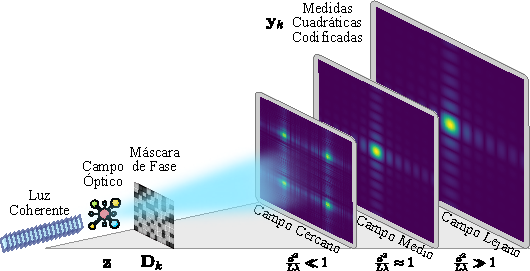
\includegraphics[width=\linewidth]{images/DiffractionSystem.pdf}
    \caption{\hspace{2mm}Sistema óptico de difracción codificado.}
    \label{fig:difraction_systems}
\end{figure}

\section{PROBLEMA DE RECUPERACIÓN DE FASE}

Debido a que los sensores únicamente captan la información de la intensidad de la luz, el modelo de adquisición en los sistemas ópticos de difracción se describe como

\begin{equation}
    \mathbf{y}_{\ell, \psi} = \vert \mathbf{A}_{\ell, \psi}\mathbf{z} \vert^2, 
    \label{eq:phase_retrieval_problem}
\end{equation}

donde $\mathbf{z} \in {\mathbb{C}}^{n}$ es una vectorización del objeto de interés, $\mathbf{y}_{\ell, \psi} \in \mathbb{R}^{n}$ son las medidas adquiridas y $\mathbf{A}_{\ell, \psi}\in\mathbb{C}^{n\times n}$ son las matrices que describe la propagación en el campo $\psi$ del frente de onda de la luz hasta el sensor, con,  $\ell=1,\dots,L$, siendo $L$ el número total de proyecciones. De acuerdo con la teoría de difracción \myfootcite{poon2014introduction}, la propagación del frente de onda del objeto se modela entre los campos, cercano, medio y lejano dependiendo del número de Fresnel $F = \frac{d^2}{L\lambda}$, que determina el modelado matemático acorde a la zona de difracción en que se captan las medidas.

% \begin{align}
%     \mathbf{y}_k= 
%          \begin{cases}
%             \vert \mathbf{FTF}^{H}\mathbf{D}_k\mathbf{z} \vert^2, & \hfill (\text{Campo Cercano, }F \ll 1, \psi=1) \nonumber, \\ 
%             \vert \mathbf{F}^{H}\mathbf{Q}\mathbf{D}_k\mathbf{z} \vert^2,  & \hfill (\text{Campo Medio, }F \approx 1, \psi=2), \\
%             \vert \mathbf{F}\mathbf{D}_k\mathbf{z} \vert^2,  & \hfill (\text{Campo Lejano, } F \gg 1, \psi=3),   \nonumber
%          \end{cases}
%     \label{eq:modelado_zonas_difraccion}
% \end{align}

\begin{equation}
    \mathbf{y}_{\ell,\psi}= \left\{\begin{matrix}
\vert \mathbf{F}\mathbf{T}\mathbf{F}^\mathcal{H} \mathbf{D}_\ell \mathbf{z} \vert^2 & \text{si } \psi=1\rightarrow \text{Campo cercano}\\ 
\vert \mathbf{F}^\mathcal{H}\mathbf{Q}\mathbf{D}_\ell \mathbf{z} \vert^2&\text{si } \psi=2\rightarrow\text{ Campo medio} \\ 
\vert \mathbf{F}\mathbf{D}_\ell \mathbf{z} \vert^2 &\text{si } \psi=3\rightarrow\text{Campo lejano}
\end{matrix}\right., \label{eq:matrix_a}
\end{equation}

donde $\vert \cdot \vert$ representa el operador de magnitud, $\mathbf{F}$ corresponde a la transformada discreta de Fourier, la matriz diagonal $\mathbf{D}_\ell \in \mathbb{C}^{n \times n}$ representa las máscaras de fase, finalmente $\mathbf{T} \in \mathbb{C}^{n \times n}$ y $\mathbf{Q} \in \mathbb{C}^{n \times n}$ son matrices ortogonales que modelan la función de transferencia espacial del campo medio y cercano, respectivamente \myfootcite{poon2014introduction,goodman2005introduction}.

\begin{figure}[H]
    \centering
    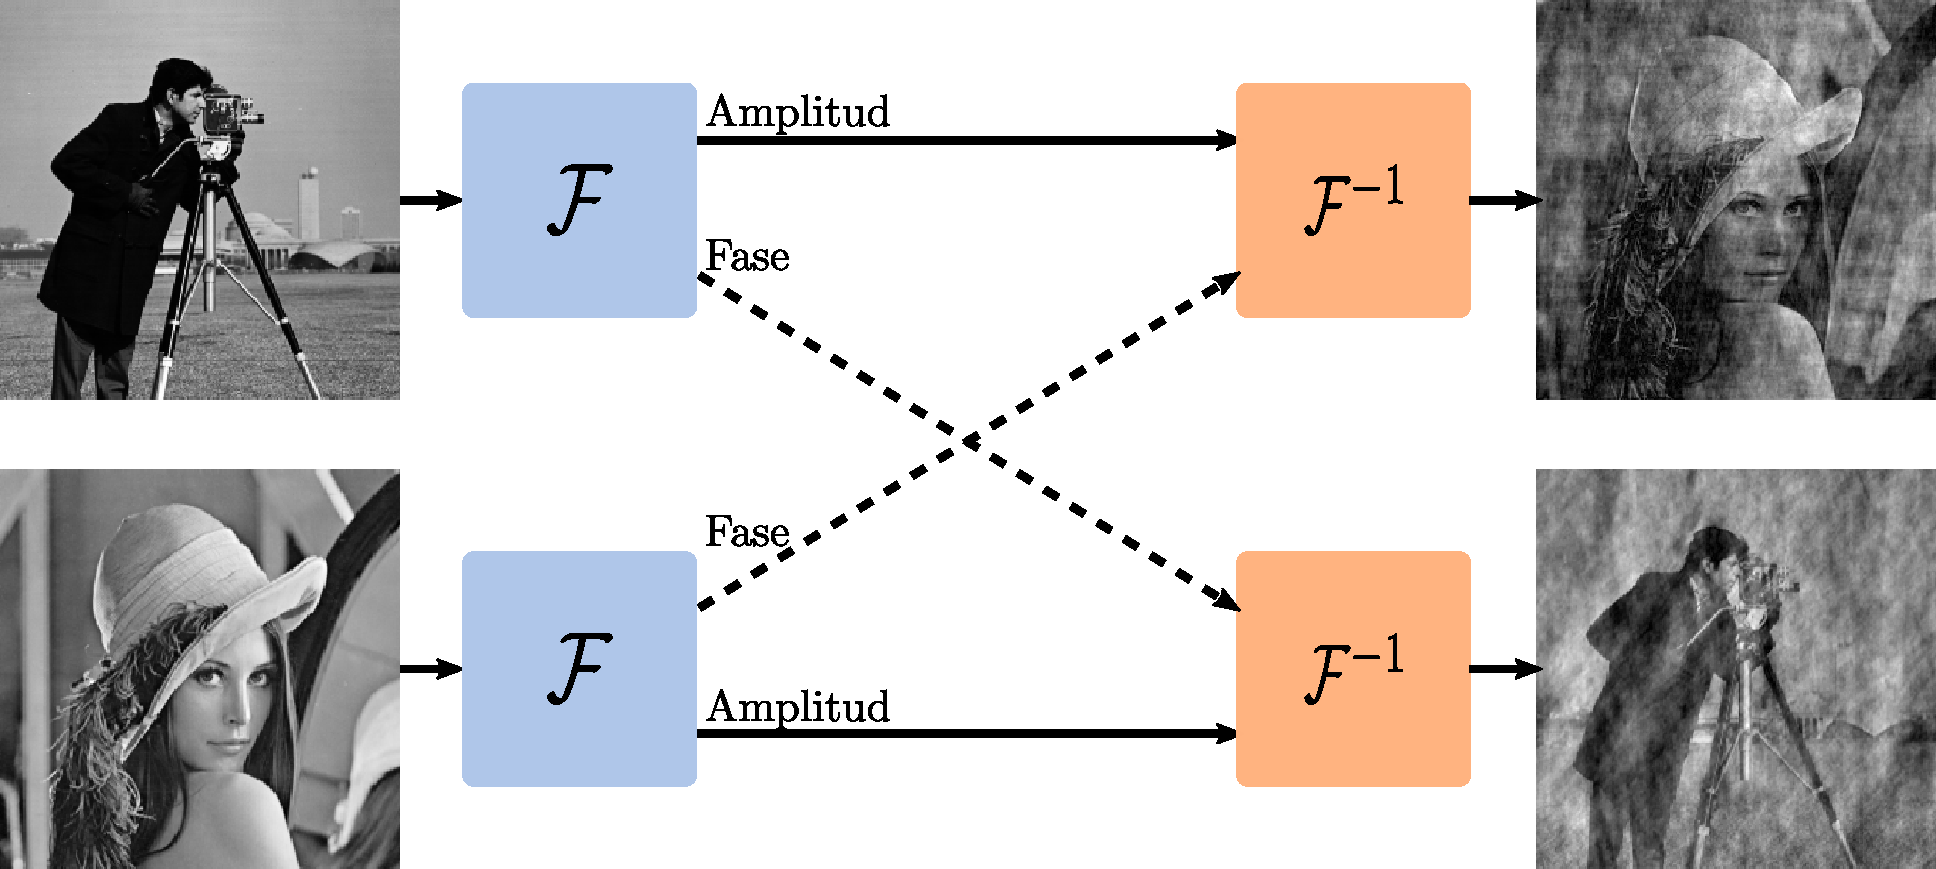
\includegraphics[width=0.8\linewidth]{images/mescla_abs_fase.pdf}
    \caption{\hspace{2mm}Experimento  intercambiando las fases de la transformada de Fourier de 2 imágenes .}
    \label{fig:mescla_fases}
\end{figure}

Cabe señalar la importancia de la información fase en Fourier a partir de la Figura \ref{fig:mescla_fases}. En esta Figura, se ilustra un experimento desarrollado en \myfootcite{shechtman2015phase} donde se intercambia la información de fase de la transformada de Fourier de dos imágenes, posteriormente, se aplica la transformada de Fourier inversa a este intercambio. En este ejemplo, se observa que en la imagen resultante predomina la información de las fases contrarias.

\section{MEDIDAS CUADRÁTICAS CODIFICADAS}
Dado la naturaleza cuadrática de la formulación en (\ref{eq:phase_retrieval_problem}), este problema se denomina como NP-difícil. Una forma de mitigar la complejidad de este problema, es incluyendo elementos de modulación de fase aleatorios en la formulación, puesto que, estas máscaras aleatorias permiten generar redundancia en las medidas, que conlleva a la obtención una solución exacta con alta probabilidad si se tienen las suficientes muestras \myfootcite{candes_CDP}.

Generalmente, las entradas aleatorias de la matriz  $\mathbf{D}_{\ell} = \mathrm{diag}(\mathbf{d})$ son $i.i.d$ copias de una variable aleatoria $d \in \mathbb{C}$ con $\mathbf{d} \in \{d\}^{n}$, donde $\mathrm{diag}(\cdot)$ devuelve una matriz diagonal cuadrada de un vector dado. Aquí, $d$ representa una modulación pasiva en la fase, se debe imponer que $d$ no aumenta la energía de la escena durante el proceso de modulación, por lo que se establece la Definición \ref{def:admissible}.

\begin{definition}{(Variable aleatorias admisible). \myfootcite{9062527}} 
    Una variable aleatoria que cumple con $|d|\leq 1$, se considera admisible como elemento de modulación en fase.\label{def:admissible}
\end{definition}


Algunos ejemplos de variables aleatorias que satisfacen la Definición \ref{def:admissible} se listan en la Tabla \ref{tab:admi_examples}. Estas variables aleatorias como elementos de codificación han sido usados en \myfootcite{9062527}.

\begin{table}[!h]
\centering
\begin{tabular}{|c|c|}
\hline
\textbf{Elemento de codificación} & \textbf{Probabilidad}                     \\ \hline
$d \in \{0, 1\}$         & $\{ \frac{1}{2},  \frac{1}{2}\}$ \\ \hline
$d \in \{-1, 1\}$        & $\{ \frac{1}{2},  \frac{1}{2}\}$ \\ \hline
$d \in \{-1, 1, -j,  j\}$ & $\{ \frac{1}{4},  \frac{1}{4}, \frac{1}{4},  \frac{1}{4}\}$ \\ \hline
\end{tabular}
\caption{Ejemplos de codificaciones aleatórias admisibles según la Definición \ref{def:admissible}.}
\label{tab:admi_examples}
\end{table}

% \begin{equation}
%     \vert d \vert \leq M, \quad \mathbb{E}[d] = 0, \quad  \mathbb{E}[d^2] = 0, \quad  \mathbb{E}[\vert d \vert^4] = 2\mathbb{E}[\vert d \vert^2]^2,    
%     \label{eq:restricciones_mascara}
% \end{equation}

% donde $\mathbb{E}[\cdot]$ corresponde al valor esperado. Aquí, se busca que $M=1$ para que la codificación no incremente la potencia de las medidas cuadráticas.

\chapter{ALGORITMOS DE RECUPERACIÓN DE FASE}
Para recuperar el campó óptico inicial a partir de medidas cuadráticas codificadas, la literatura ha planteado diferentes algoritmos basados en formulaciones convexas y no convexas.

\section{FORMULACIONES CONVEXAS}

Estos tipo de algoritmos relajan el problema recuperación de fase a un problema convexo equivalente.

\begin{itemize}
    \item \textbf{PhaseLift \myfootcite{candes2013phaselift}}:
    Este algoritmo plantea el problema de recuperación de la fase como una minimización de la traza de la siguiente forma
    \begin{equation}
        \begin{aligned}
            \minimize_{\mathbf{z} \in \mathbb{C}^{n}} \quad & \quad \mathrm{Traza}(\mathbf{z}\mathbf{z}^{\mathcal{H}}), \\
            \subjectto \quad & \quad \mathcal{A}(\mathbf{z}\mathbf{z}^{\mathcal{H}}) = \mathbf{b}, \\
             &\quad  \mathbf{z}\mathbf{z}^{\mathcal{H}} \succ 0,
        \end{aligned}
    \end{equation}
    
    donde $\mathcal{A}( \cdot ): \mathbb{R}^{n} \rightarrow \mathbb{R}^{m}$ es un operador lineal y $\mathrm{Traza}(\cdot)$ representa la traza de una matriz.
    
    \item \textbf{PhaseMax} \myfootcite{goldstein2018phasemax}:
    Sea $\mathbf{\hat{z}} \in \mathbb{C}^{n}$ un vector aproximación de la señal original $\mathbf{z}$, de modo que, la señal reconstruida se obtiene solucionando el siguiente problema convexo
        
    \begin{equation}
        \begin{aligned}
            \maximize_{\mathbf{z}\in \mathbb{C}^n} \quad & \langle \mathbf{z}, \mathbf{\hat{z}} \rangle_{\mathbb{R}}, \\
            \subjectto \quad & \vert \langle \mathbf{a}_i,\mathbf{z} \rangle \vert \leq (\boldsymbol{\phi})_i,
        \end{aligned}
    \end{equation}
    donde $\langle \cdot, \cdot \rangle_{\mathbb{R}}$ denota la parte real del producto interno y $(\boldsymbol{\phi})_i = \sqrt{(\mathbf{y})_i}$
    
\end{itemize}

\section{FORMULACIONES NO CONVEXAS}
Las formulaciones no convexas calculan el gradiente siguiendo la diferenciación de Wirtinger como los mostrados a continuación.
\begin{itemize}
    \item \textbf{TRUNCATED WIRTINGER FLOW (TWF):}
    El algoritmo TWF propuesto en \myfootcite{chen2017solving}, basa el modelo de muestreo según un variables aleatorias que siguen una distribución de Poisson de la forma:
    
    \begin{equation}
        (\mathbf{y})_i\sim \mathrm{Poisson}( \vert \langle \mathbf{a}_i,\mathbf{z}\rangle \vert^2 ), \quad i=1,\dots,m.
    \end{equation}
    
    TWF busca minimizar la máxima estimación de probabilidad 
    
    \begin{equation}
        \minimize_{z \in \mathbb{C}^{n}} - \sum_{i=1}^{m} \ell(\mathbf{z};\mathbf{y}_i),
    \end{equation}
    
    donde $\ell(\mathbf{z};\mathbf{y}_i) = { \mathbf{y}_i\log(|\mathbf{a}_i^H \mathbf{z}|^2) -|\mathbf{a}_i^H \mathbf{z}|^2 }$ con $(\cdot)^H$ el operador de conjugada transpuesta
    
    \item \textbf{TRUNCATED AMPLITUDE FLOW (TAF):}

    El algoritmo TAF \myfootcite{wang2017solving} adopta un criterio de mínimos cuadrados para recuperar $\mathbf{z}$ basado en las medidas sin fase $\mathbf{y}$ 
    
    \begin{equation}
        \minimize_{\mathbf{z} \in \mathbb{C}^{n}} \frac{1}{2m} \sum_{i=1}^{m} (\vert \langle \mathbf{a}_i,\mathbf{z}\rangle \vert - (\boldsymbol{\phi})_i)^2,
    \end{equation}
    
    Este algoritmo asume que las medidas $\mathbf{y}_i$ provienen de un sistema gaussiano de la forma $\mathbf{y}_i \sim \mathcal{N}(\vert \langle \mathbf{a}_i,\mathbf{z}\rangle \vert^2, 1)$
    
    \item \textbf{REWEIGHTED AMPLITUDE FLOW (RAF):}

    El algoritmo RAF formulado en \myfootcite{wang2018phase} sigue el criterio de maximizar la estimación de probabilidad de la forma
    
    \begin{equation}
        \minimize_{z \in \mathbb{C}^{n}} -\sum_{i=1}^{m} \ell(\mathbf{z};(\boldsymbol{\phi})_i/(\mathbf{y})_i),
    \end{equation}
    
    donde en el caso de un muestreo con ruido gaussiano basado en la amplitud $\ell(\mathbf{z};\mathbf{y}_i) = (\vert \langle \mathbf{a}_i,\mathbf{z}\rangle \vert - (\boldsymbol{\phi})_i)^2$ o basado en la intensidad  $\ell(\mathbf{z};(\mathbf{y})_i) = (\vert \langle \mathbf{a}_i,\mathbf{z}\rangle \vert^2 - (\mathbf{y})_i)^2$. Por otra parte, basado en un muestreo con distribución de Poisson, $\ell(\mathbf{z};(\mathbf{y})_i) = {(\mathbf{y})_i \log(|\mathbf{a}_i^H \mathbf{z}|^2) -|\mathbf{a}_i^H \mathbf{z}|^2 }$ 
\end{itemize}





\chapter{SISTEMAS DE CLASIFICACIÓN}

La clasificación ha sido una de las tareas computacionales más abordadas en el estado del arte. Específicamente, los algoritmos de clasificación se pueden separar en los más tradicionales como las SVM y KNN \myfootcite{kim12012comparing} y los algoritmos basados en redes neuronales que recientemente han dominado diferentes campos \myfootcite{li2019deep,li2018deep, wang2019development}
\section{MÁQUINAS DE SOPORTE VECTORIAL}
Las máquinas de soporte vectorial (SVM, por su sigla en inglés) \myfootcite{suthaharan2016support} son un método de clasificación binaria, donde cada punto $n$ dimensional $\mathbf{x}_i$ le corresponde una etiqueta de clase $c_i \in \{1,-1\}$.

Suponiendo que los datos de ambas clases son separables linealmente, este método propone separar los datos usando el hiper plano $\mathbf{w}\mathbf{x}_i + b = 0$. En la Figura \ref{fig:svm}, se muestra una representación de una SVM en $\mathbb{R}^2$

\begin{equation}
    \begin{split}
        \mathbf{w}\mathbf{x}_i + b &\geq 1 \quad si \quad c_i=1, \\
        \mathbf{w}\mathbf{x}_i + b &\leq 1 \quad si \quad c_i=-1.
    \end{split}
\end{equation}

Cabe resaltar que para todos los elementos del conjunto de datos se cumple que:

\begin{equation}
    c_i(\mathbf{w}\mathbf{x}_i + b) \geq 1, \quad i=1,\dots, m
\end{equation}

\begin{figure}[H]
    \centering
    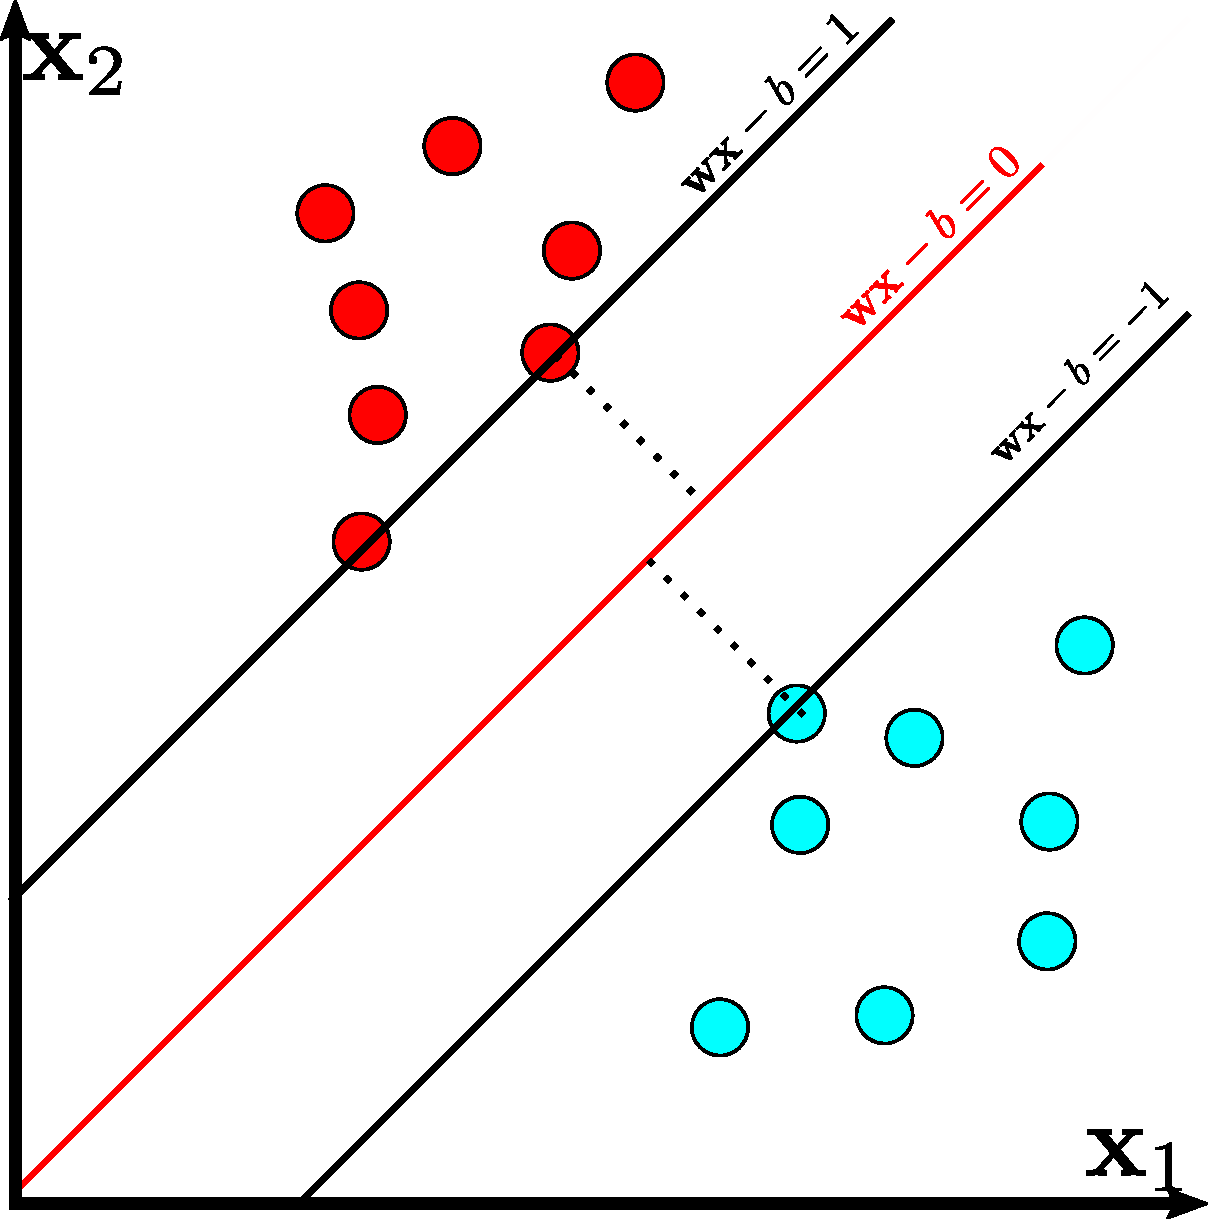
\includegraphics[width=0.4\linewidth]{images/svm.pdf}
    \caption{\hspace{2mm}Representación de una SVM en $\mathbb{R}^2$. La recta $\mathbf{wx} -b = 0$ en rojo representa el plano óptimo que soluciona el problema de optimización (\ref{eq:problema_optimización_svm}).}
    \label{fig:svm}
\end{figure}

El problema de optimización se plantea de la siguiente forma:

\begin{equation}
    \begin{aligned}
        \minimize_{\mathbf{w}} & \quad \Vert \mathbf{w} \Vert, \\
        \subjectto_{\quad i=1,\dots, m} & \quad c_i(\mathbf{w}\mathbf{x}_i + b) \geq 1.
    \end{aligned}
    \label{eq:problema_optimización_svm}
\end{equation}

Usualmente no es posible separar los datos linealmente, por esta razón, se puede incluir una función no lineal $ \phi$ que transforme los datos a un conjunto de características donde las clases sean separables linealmente. El problema de optimización para una SVM usando un kernel $\phi$ se formula como

\begin{equation}
    \begin{aligned}
        \minimize_{\mathbf{w}} & \quad \Vert \mathbf{w} \Vert, \\
        \subjectto_{\quad i=1,\dots, m} & \quad c_i(\mathbf{w}\phi(\mathbf{x}_i) + b) \geq 1.
    \end{aligned}
\end{equation}


\section{K VECINOS MÁS CERCANOS}

K vecinos más cercanos (KNN, por sus siglas en inglés) propone que un conjunto $D = \{(\mathbf{x}_i, c_i)\}_1^n$, siendo $\mathbf{x}_i$ el vector de características e $c_i$ la clase correspondiente. Para un nuevo vector a clasificar $\mathbf{\hat{x}}$, el algoritmo KNN encuentra los $K$ puntos más cercanos del dataset. La Figura \ref{fig:knn} muestra una representación de la clasificación de dos nuevas muestras en $\mathbb{R}^2$ con $K = 5$. Usualmente la función de distancia usada corresponde a la distancia euclidiana

\begin{equation}
    d(\mathbf{x}_p,\mathbf{x}_q) = \Vert \mathbf{x}_p-\mathbf{x}_q \Vert_2
    \label{eq:distancia_euclidiana}
\end{equation}

\begin{figure}[H]
    \centering
    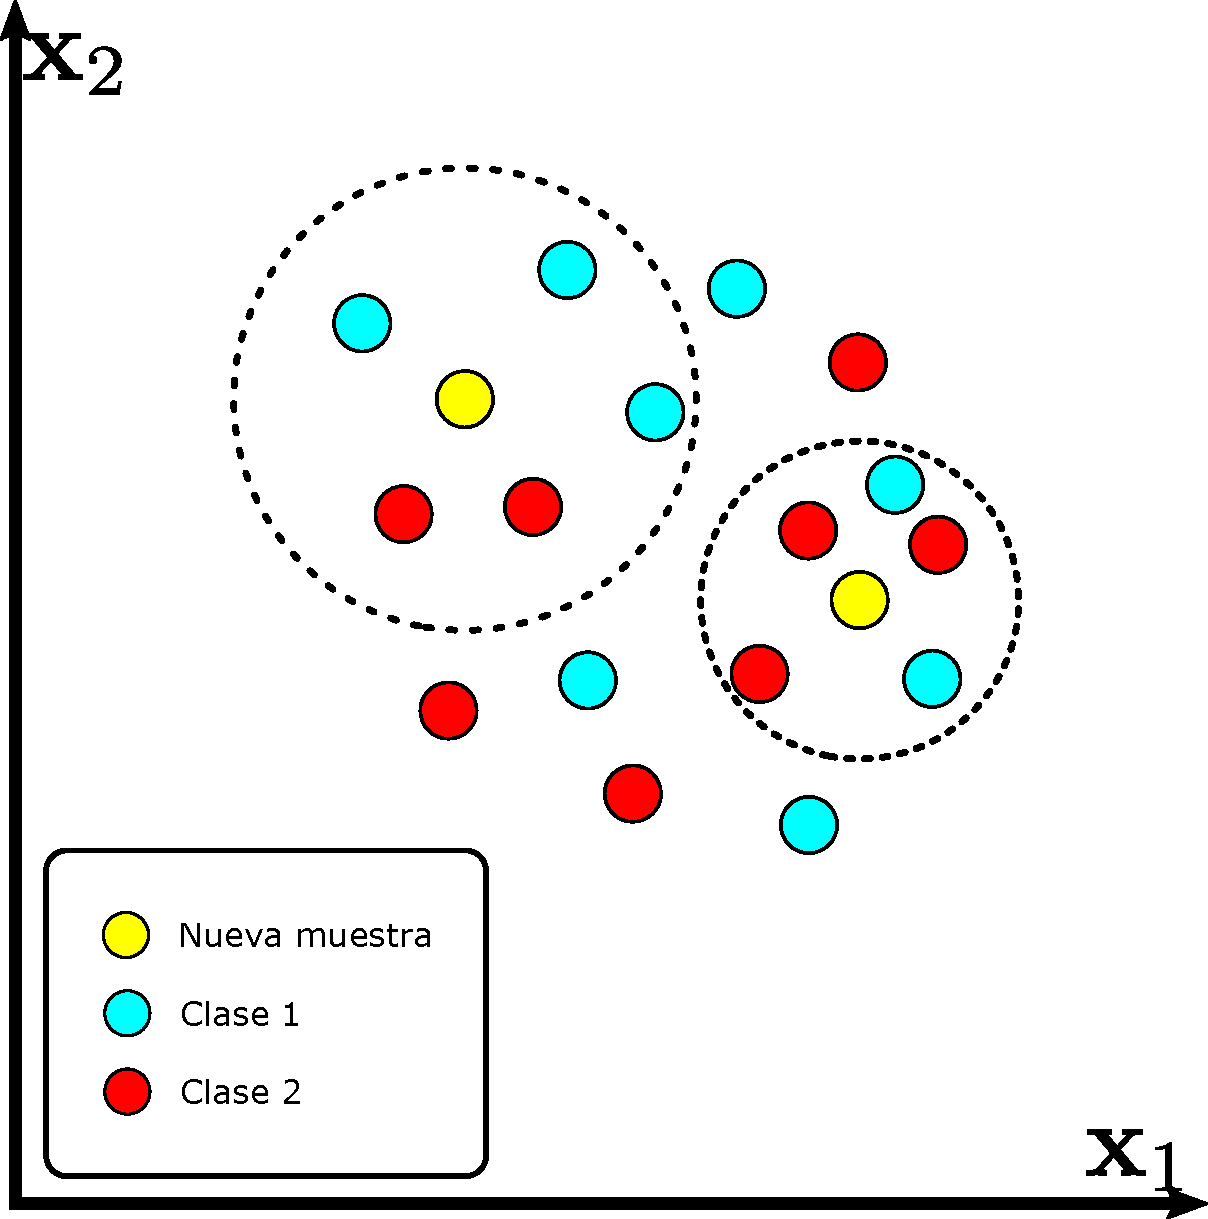
\includegraphics[width=0.4\linewidth]{images/knn.pdf}
    \caption{\hspace{2mm}Representación de KNN en $\mathbb{R}^2$ con $K = 5$.}
    \label{fig:knn}
\end{figure}

Posteriormente, haciendo uso de las clases de los $K$ puntos encontrados, de tal forma que $C \subset D$ y $\vert C \vert = K$, se cuantifica la cantidad de veces que aparece cada clase y se clasifica la nueva muestra $\mathbf{\hat{x}}$ con la clase que más veces aparezca de la forma

\begin{equation}
    \mathrm{clase}(\mathbf{\hat{x}}) =  \argmax_{\hat{c}} \bigg\{ \sum_{\hat{c} \in C} \delta(C,\hat{c})\bigg\},
\end{equation}

donde $\delta(\cdot,\cdot)$ corresponde a la función delta de Kronecker, dada por

\begin{equation}
    \delta(a,b) = \begin{cases}
        1, \quad a = b \\
        0, \quad a \neq b
    \end{cases}
\end{equation}
\section{REDES NEURONALES}

Los enfoques de aprendizaje profundo han generado un gran progreso en problemas muy complejos en los últimos años
\myfootcite{he2016deep,li2019deep,li2018deep, wang2019development,vaswani2017attention}. El aprendizaje profundo busca encontrar una función $f: \mathbb{R}^{d_1} \rightarrow \mathbb{R}^{d_2}$. La función $f$ se suele llamar arquitectura de red neuronal profunda, puesto que, consiste en la concatenación de múltiples capas compuestas de unidades mínimas llamadas neuronas. Cada neurona realiza una combinación lineal entre las entradas, para posteriormente usar una función no lineal en la salida. Las salidas de cada neurona en una capa funcionan como entrada de las neuronas ubicadas en la siguiente capa, creando así, una arquitectura de red neuronal profunda \myfootcite{fan2019selective}. En la Figura \ref{fig:nn}, se muestra una arquitectura de una arquitectura de red neuronal $f: \mathbb{R}^{d_1} \rightarrow \mathbb{R}^{d_2}$

\begin{figure}[H]
    \centering
    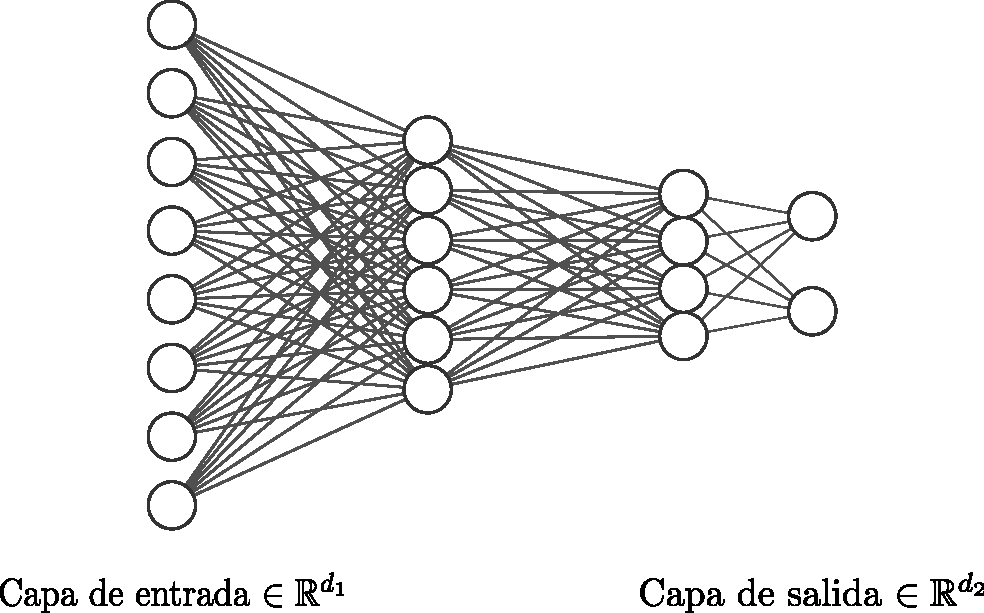
\includegraphics[width=0.6\linewidth]{images/nn.pdf}
    \caption{\hspace{2mm}Arquitectura de una arquitectura de red neuronal $f: \mathbb{R}^{d_1} \rightarrow \mathbb{R}^{d_2}$.}
    \label{fig:nn}
\end{figure}

En la ecuación. (\ref{eq:red_neuronal}), se muestra el modelado matemático de una red neuronal sencilla. 
\begin{equation}
    \footnotesize 
    \big\{f_\theta(\mathbf{x}) = \sigma_{L}(\mathbf{W}_{L}\sigma_{L-1}(\mathbf{W}_{L-1} (\dots \sigma_2(\mathbf{W}_2\sigma_1(\mathbf{W}_1\mathbf{x})))) \quad \vert \quad\theta = \{\mathbf{W}_{1} \dots \mathbf{W}_{L}\}  \big\},
    \label{eq:red_neuronal}
\end{equation}

donde para cada capa $1 \leq \ell \leq L$, $\sigma_\ell$ corresponde a una función no lineal en dicha capa y $\mathbf{W}_\ell$ La matriz de pesos. Para entrenar los pesos $\theta$ bajo un enfoque de aprendizaje supervisado, este método hace uso de un conjunto de entrenamiento $\{(\mathbf{x}_i, c_i) \}_{i=1}^{N}$ y una función de costo $\mathcal{L}( c_i,  f_\theta(\mathbf{x}_i))$ para plantear el problema de optimización 

\begin{equation}
    \minimize_\theta \frac{1}{N}\sum_{i=1}^{N} \mathcal{L}( c_i,  f_\theta(\mathbf{x}_i))
    \label{eq:optimización_nn}
\end{equation}

\section{CLASIFICACIÓN USANDO MEDIDAS CUADRÁTICAS}
En el campo de tomografía computarizada \myfootcite{douarre2020value} e imágenes de un solo píxel \myfootcite{bacca2020coupled}, se han propuesto sistemas de clasificación que usan únicamente medidas obtenidas a través del sistema lineal de adquisición, esto debido al enfoque basado en el aprendizaje profundo en el que la arquitectura incluye una capa con el sistema óptico de adquisición. Este enfoque ha sido estudiado igualmente en imágenes difractivas como en holografía \myfootcite{kim2018deep} y cristalografía de rayos-x \myfootcite{ziletti2018insightful}, donde las medidas obtenidas son difícilmente reconocidas por el ojo humano. 

Sin embargo, estos enfoques propuestos no han sido abordados en imágenes de medidas cuadráticas codificadas, de modo que, este trabajo propone el desarrollo de un algoritmo de clasificación usando medidas cuadráticas codificadas basado en aprendizaje profundo. 


\section{CLASIFICACIÓN DE IMÁGENES USANDO REDES NEURONALES ÓPTICAS}


Recientemente, se han publicado avances en el campo de redes neuronales implementadas físicamente haciendo uso de propiedades ópticas. Este tipo de redes resaltan debido al hecho que si se realiza la inferencia de manera óptica, la velocidad de cálculo está limitada por la velocidad de la luz en el medio y no requieren una fuente de energía activa para realizar los cálculos. Específicamente en \myfootcite{lin2018all} implementan las capas de una red neuronal haciendo uso de materiales difractados, realizando la modulación de la luz en la fase y aprovechando la propagación del campo óptico para realizar tareas de clasificación


\begin{figure}[!h]
    \centering
    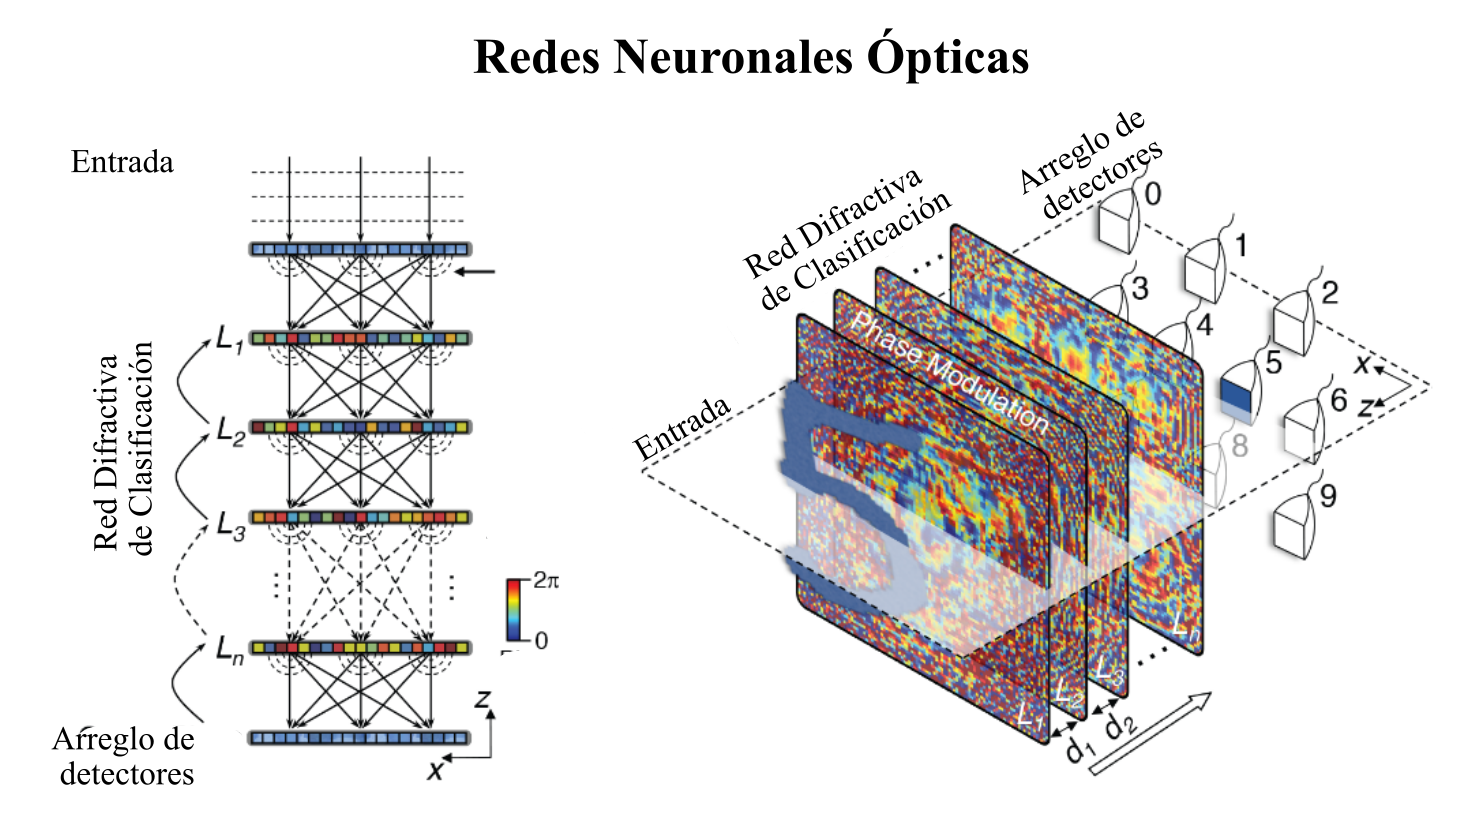
\includegraphics[width = 1\linewidth]{images/diffractive_networks.png}
    \caption{Implementación de redes neuronales ópticas implementadas ópticamente mediante elementos ópticos difractivos. Fuente: Modificado de \textit{All-optical machine learning using diffractive deep neural networks, 2018.}}
    \label{fig:optical_networks}
\end{figure}

 % Marco de referencia
% ------------------------------------------------------------------------
% ------------------------------------------------------------------------
% ------------------------------------------------------------------------
%                                Capítulo 3
% ------------------------------------------------------------------------
% ------------------------------------------------------------------------
% ------------------------------------------------------------------------

\chapter{Metodología}

El enfoque de red neuronal profunda propuesto para la clasificación de objetos desde medidas cuadráticas codificadas incluye tres etapas principales: (i) capa de adquisición, (ii) enfoque de inicialización, (iii) y red de clasificación. La Figura \ref{fig:esquema_entrenamiento} ilustra el esquema de red neuronal profunda propuesto. Primero, una capa de adquisición simula el proceso de medición \eqref{eq:phase_retrieval_problem}, donde la capa realiza un modelo de propagación del campo óptico. Luego, un procedimiento de inicialización aproxima el campo óptico $\mathbf{x}$, finalmente, la red de clasificación infiere la clase correspondiente a cada medida cuadrática codificada.


\begin{figure*}[!h]
    \centering
    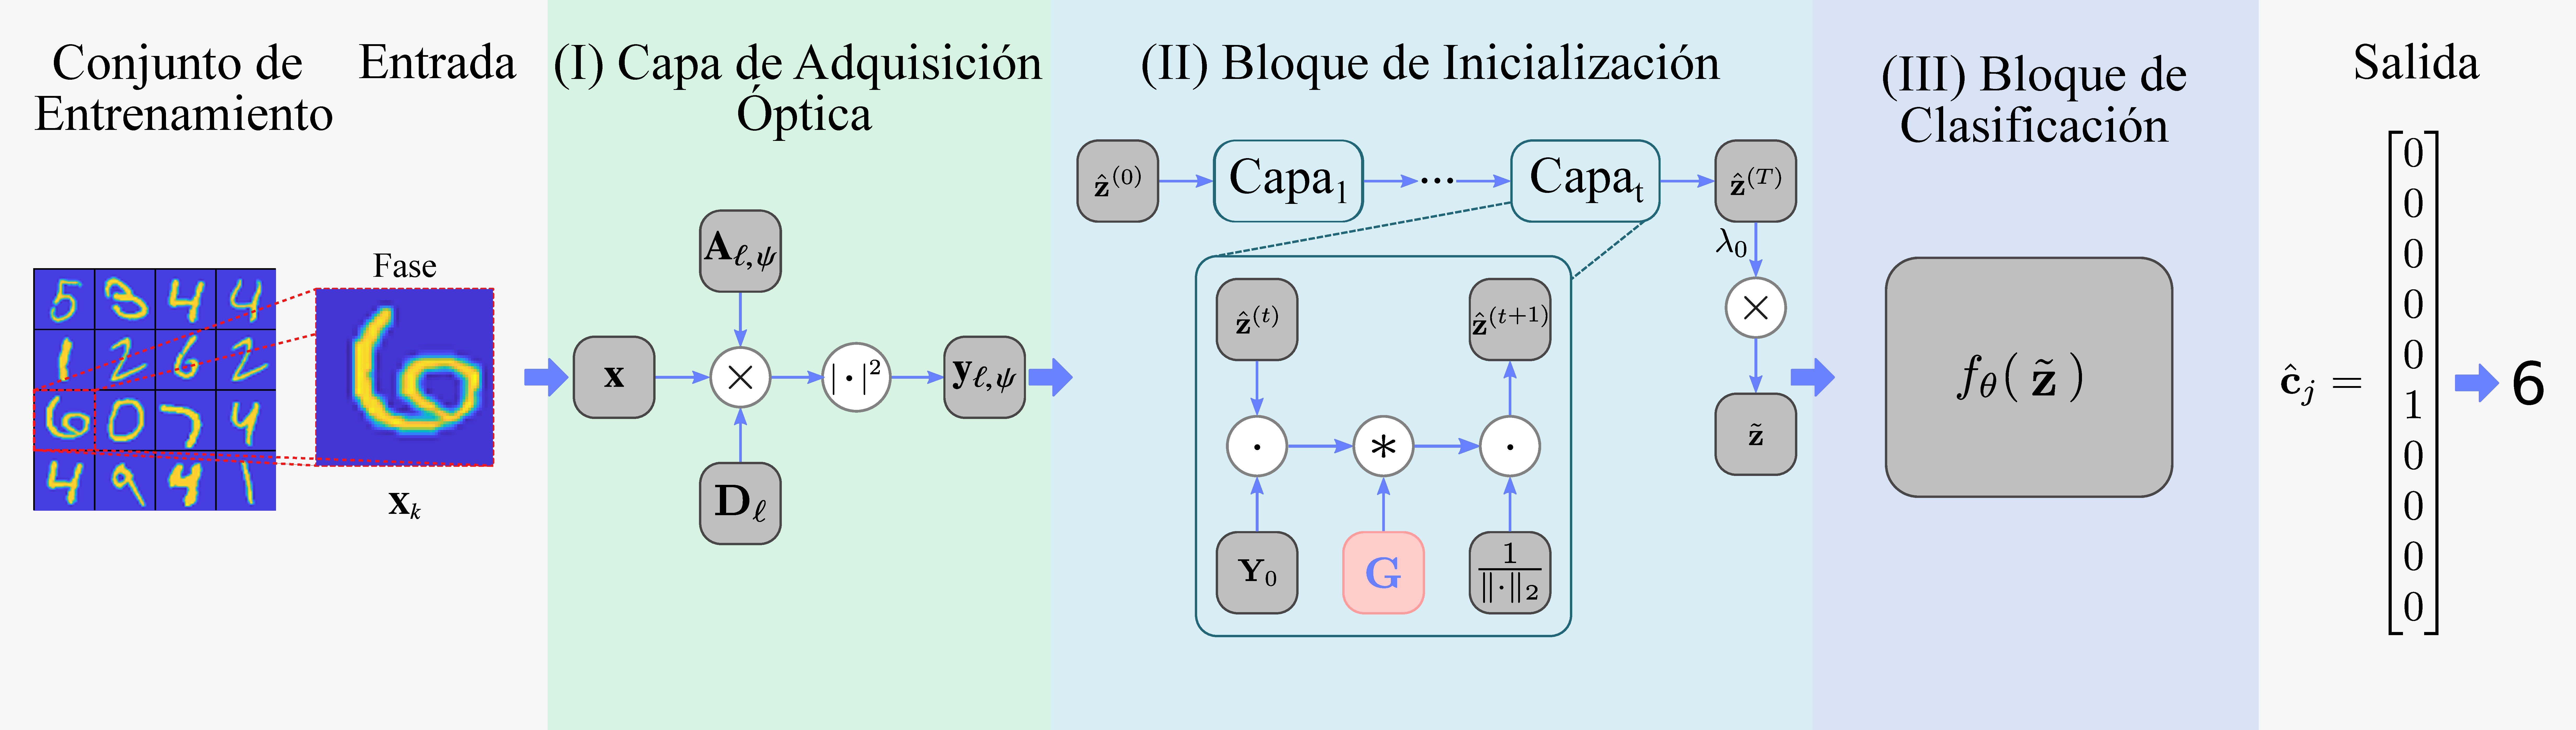
\includegraphics[width=\linewidth]{images/esquema_entrenamiento.pdf}
    \caption{Esquema de red neuronal profunda de tres etapas propuesto para la clasificación de objetos desde medidas cuadráticas codificadas.}
    \label{fig:esquema_entrenamiento}
\end{figure*}


\section{Bloque de inicialización}

Para realizar la etapa de inicialización del campo óptico, este trabajo toma ventaja del hecho de que la matriz de adquisición $\mathbf{A}_k$ es conocida, por lo tanto, se crea un mapeo $\mathcal{B}(\cdot)$ que pasa de las medidas $\mathbf{y}_k$ a una aproximación más cercana del campo óptico $\mathbf{x}$, dada por el desenvolvimiento de un algoritmo tradicional y un conjunto de capas convolucionales, de tal forma que $\hat{\mathbf{x}}=\mathcal{B}(\mathbf{A}_k, \mathbf{y}_k)$. 

% El primer enfoque usa el operador de propagación hacia atrás inverso $\mathcal{P}_\ell:\mathbb{C}^n\rightarrow \mathbb{C}^n$ del campo óptico para aproximar$\hat{\mathbf{x}}$  \myfootcite{katkovnik2017computational}, que viene dado por

% \begin{equation}
%     \hat{\mathbf{x}}= \frac{1}{L}\sum_{\ell=1}^{ L} \mathcal{P}_\ell(\mathbf{y}_\ell).
%     \label{eq:back_propagation}
% \end{equation}

Más concretamente este enfoque aplica un desenvolvimiento del algoritmo de inicialización de filtrado espectral (FSI\myfootcite{jerez2020fast}, por sus siglas en inglés). Esta inicialización se basa en un método de iteración de potencia para aproximar el campo óptico desde patrones codificados de difracción, el cual se resume en el Algoritmo \ref{alg_1}.

\begin{algorithm}[!h]
    %\scriptsize
    \caption{Algoritmo FSI}%\label{fsi_algo}
    \textbf{Entrada:} Matriz de sensado y medidas adquiridas $\{(\mathbf{A}_\ell;\mathbf{y}_\ell)\}_{\ell=1}^L$, máximo número de iteraciones $T$ y el filtro pasa bajas $ \mathbf{G}$.\newline
    \textbf{Salida:} $\hat{\mathbf{x}}$.
    \begin{algorithmic}[1]
        \State{$\tilde{\mathbf{x}}^{(0)} \leftarrow$ Aleatoriamente escogido}
        \State{ $ {\nu_\Xi}_\ell \left( \left( \mathbf{y}_\ell \right)_{i} \right) = 
                \begin{cases}
                1 & i \in \Xi_\ell \\
                0 & \text{De otra forma } \\
                \end{cases},1\leq i\leq n $
                }
        \State{ $ \tilde{\mathbf{y}}_\ell = \left[ {\nu_\Xi}_\ell \left( \left( \mathbf{y}_\ell \right)_1 \right),\cdots,{\nu_\Xi}_\ell \left( \left( \mathbf{y}_\ell \right)_n \right) \right]^T$ \Comment{Truncamiento por umbral} }
        \For{$t = 0: T-1$ }
        \State{$\tilde{\mathbf{x}}^{(t+1)} \leftarrow \sum_{\ell=1}^{L}\mathcal{P}_\ell\left(  \tilde{\mathbf{y}}_\ell \odot \mathbf{A}_\ell  \tilde{\mathbf{x}}^{(t)} \right) $ }
        \State{$\tilde{\mathbf{x}}^{(t+1)} \leftarrow {\mathbf{G}} * \tilde{\mathbf{x}}^{(t)}$\Comment{Operador de convolución}}
        
       \State{$\tilde{\mathbf{x}}^{(t+1)} \leftarrow \frac{\tilde{\mathbf{x}}^{(t+1)}}{{\Vert \tilde{\mathbf{x}}^{(t+1)} \Vert}_2 }$	\Comment{Normalización}}
        \EndFor
        \State{$\hat{\mathbf{x}}^{(T)} =  \tilde{\mathbf{x}}^{(T)} \sqrt{\frac{\sum_{\ell=1}^{L} \Vert\mathbf{y}_\ell \Vert_{2}^2 }{nL} } $\Comment{Escalado}}
    \end{algorithmic}
    \label{alg_1}
\end{algorithm}

El algoritmo FSI crea el conjunto de índices $\Xi_\ell$ correspondientes a los valores más grandes de $\{(\mathbf{y}_\ell)_{i}/\vert \vert\mathbf{a}_{\ell,i}\vert \vert_2\}$, donde $\mathbf{a}_{\ell,i}\in\mathbb{C}^{n}$ representan las filas de $\mathbf{A}_\ell$. Adicionalmente, el algoritmo incluye un filtro $\mathbf{G}$, el cual fue implementado como una capa convolucional, de tal manera que cada iteración del algoritmo FSI se aplica un filtrado que promueve mejoría en la aproximación, por lo tanto una mejora en la clasificación. 
\section{Bloque de clasificación}

En este trabajo se hizo uso de diferentes arquitecturas de clasificación del estado del arte. \textcolor{red}{Explicar cada una?} de red de clasificación MobilNetV2 \myfootcite{sandler2018mobilenetv2} como la red de clasificación $f_\theta(\cdot)$. La Figura. \ref{fig:mobilnetv2} ilustra la arquitectura usada. La entrada pasa a través de una capa convolucional con 32 canales, luego, 7 bloques residuales de cuello de botella reducen la dimensión de los datos y aumentan el número de canales para extraer las características. Finalmente, la capa convolucional resultante toma una entrada con forma de $1\times1\times1280$ para aplicar filtros convolucionales de $1\times1$ con el número de canales igual al numero de clases en el dataset.

\begin{figure}[!h]
    \centering
    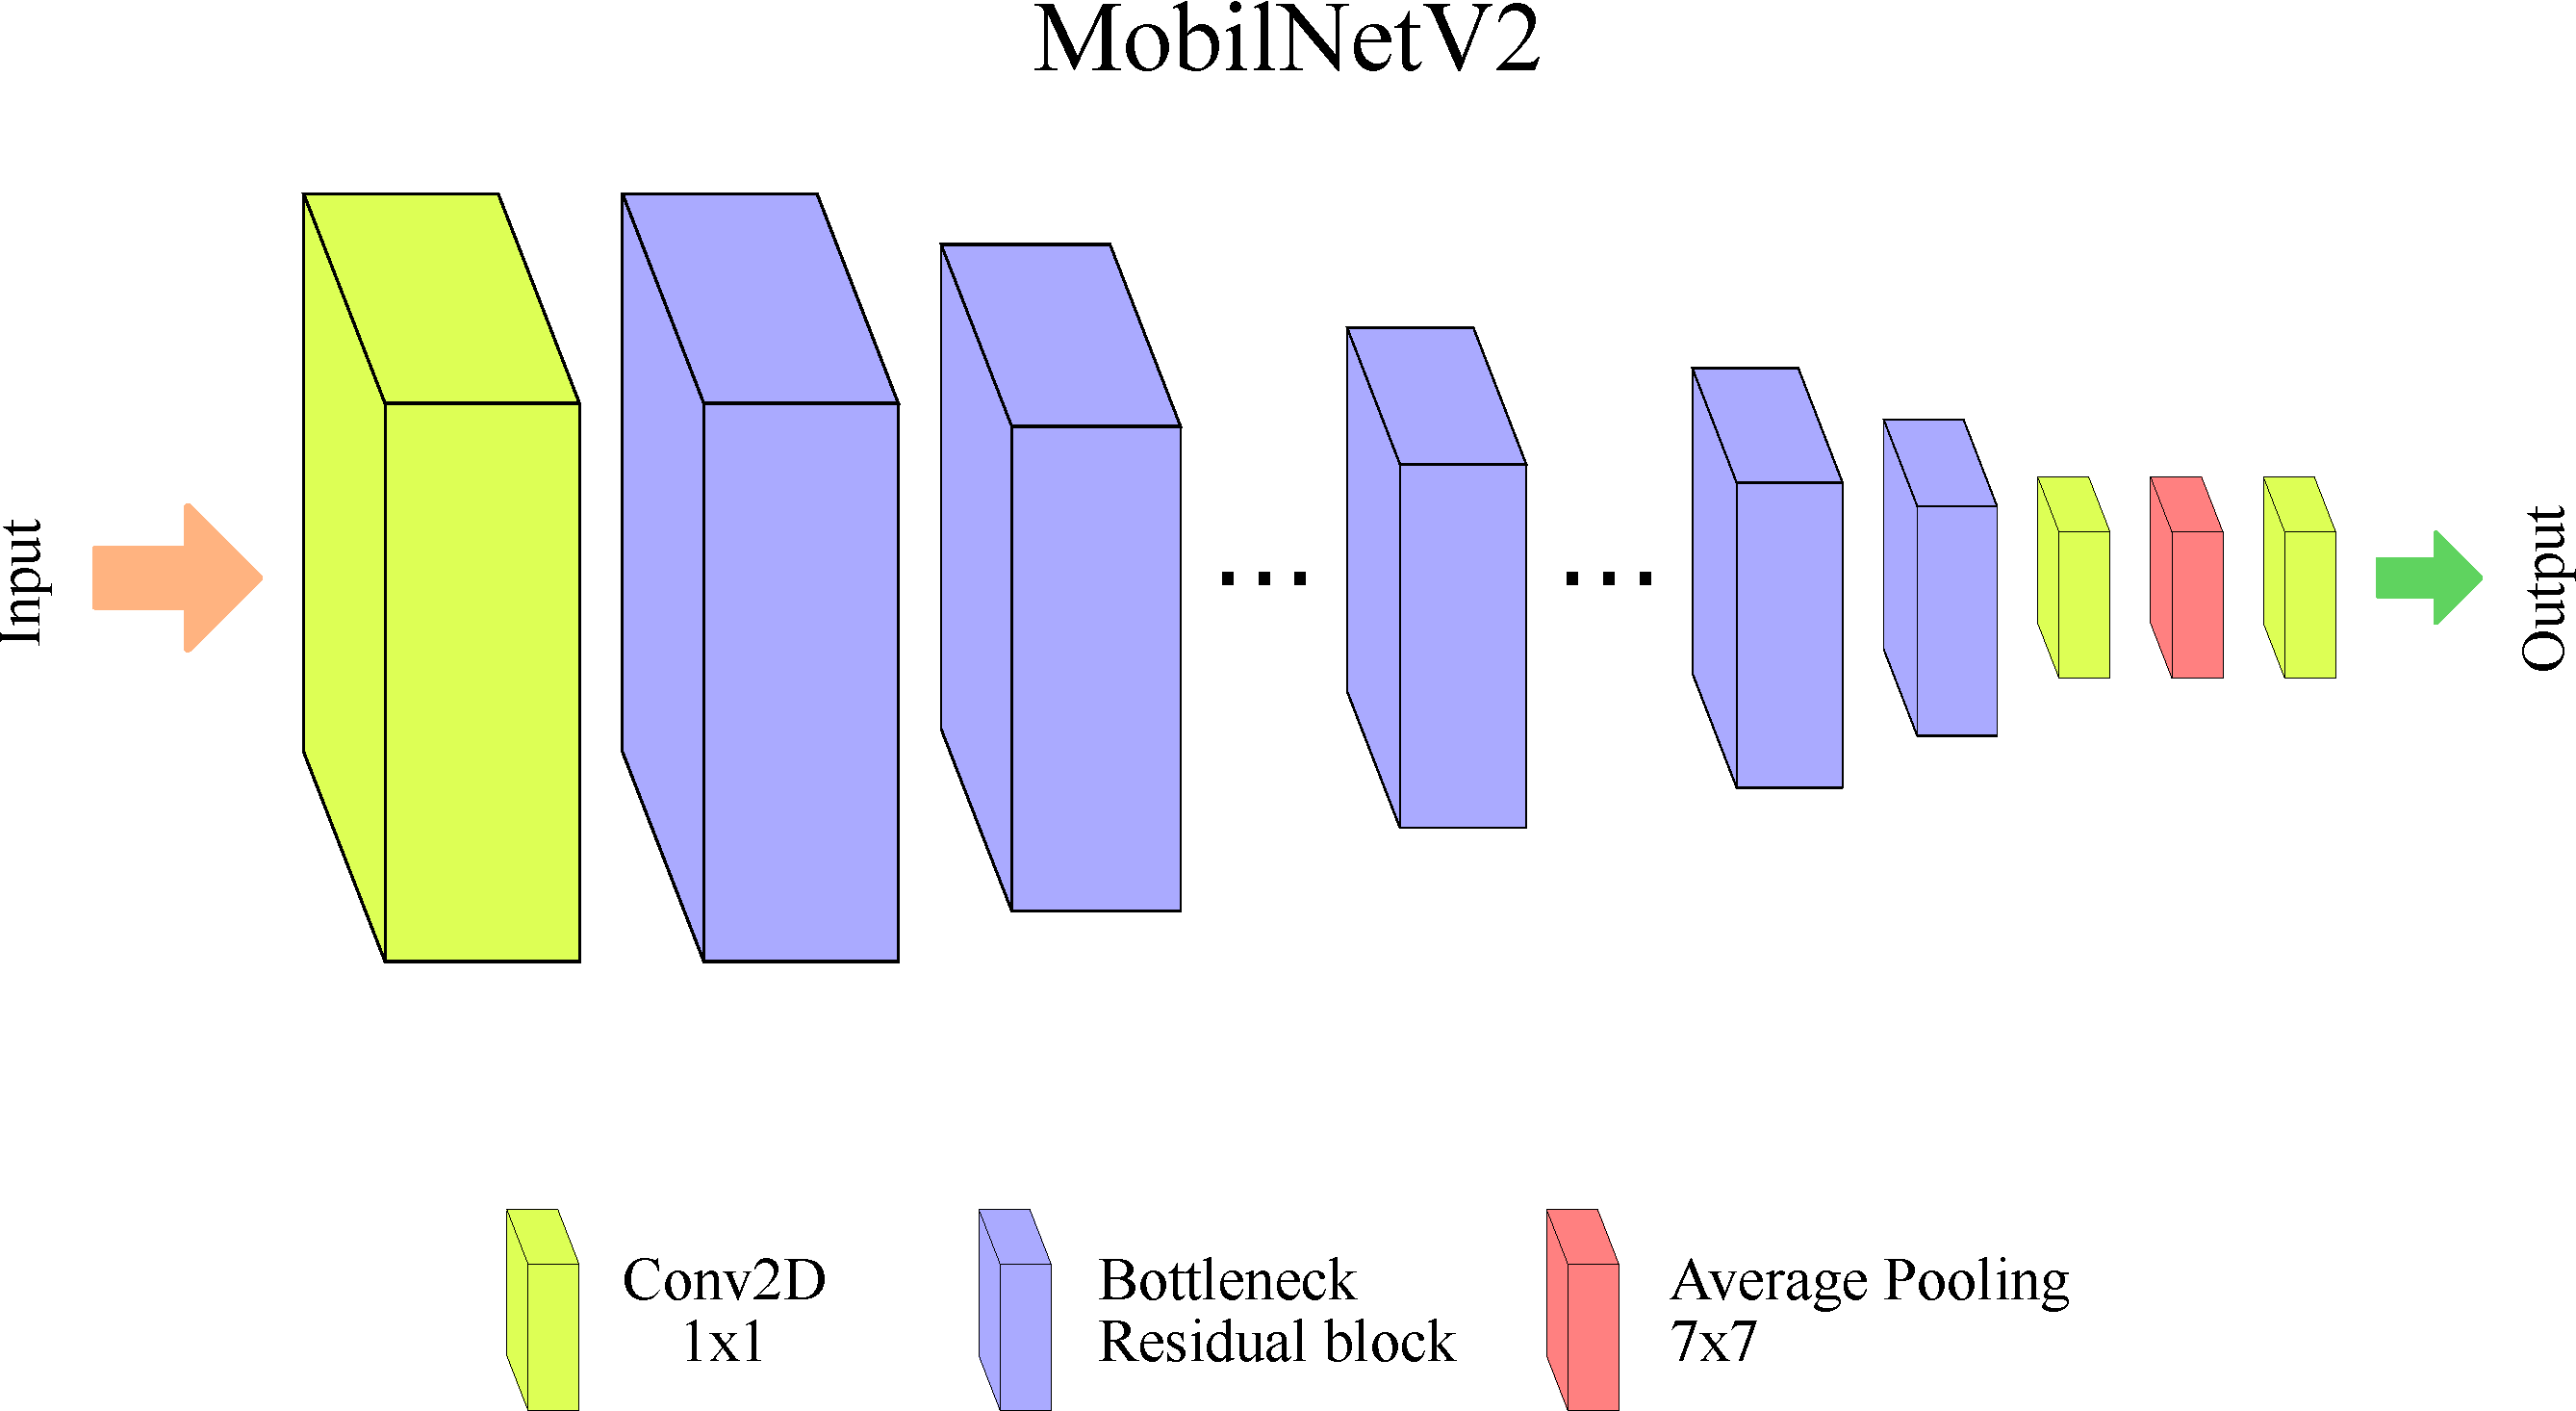
\includegraphics[width=1\linewidth]{images/MobilNet.pdf}
    \caption{Arquitectura de red MobilnetV2.}
    \label{fig:mobilnetv2}
\end{figure}

Para entrenar los pesos $\theta$ de la red de clasificación $f_\theta(\cdot)$, se puede usar el siguiente problema de optimización

\begin{equation}
    \mathbf{\theta}^* \in  \argmin_{\mathbf{\theta}} \frac{1}{J}\sum_{j = 1}^{J} \mathcal{L}\left( c^{(j)}, f_{\mathbf{\theta}}\left(\mathcal{B}(\mathbf{y}_{\ell}^{(j)})\right)\right).
    \label{eq:dl_optimization}
\end{equation}

Este problema minimiza la función pérdida usualmente llamada entropía categórica cruzada $\mathcal{L}(\cdot, \cdot)$ entre las etiquetas del dataset $c^{(j)}$, y las clases predichas $\hat{c}^{(j)} = f_\theta(\mathcal{B}(\mathbf{y}_\ell^{(j)}))$, donde $J$ es el número total de medidas y $\mathbf{y}_\ell^{(j)}$ es la medida cuadrática codificada al  j-ésimo ejemplo.


\subsection{Entrenamiento del esquema propuesto}

El Algoritmo \ref{alg:algoritmo_2} resume el proceso de entrenamiento del esquema mostrado en la Figura \ref{fig:esquema_entrenamiento},  Para entrenar el esquema propuesto. Inicialmente, en la línea 2, el filtro de inicialización es inicializado usando una distribución uniforme $\mathcal{U}(\mathbf{0},\mathbf{1})$. Luego, el modelo de propagación descrito por la Ecuación \eqref{eq:phase_retrieval_problem} es simulado por la capa de adquisición en la línea 5. Posteriormente se realiza el proceso de inicialización el cual aproximará las medidas cuadráticas codificadas al campo óptico inicial en la línea 6. Para obtener una clasificación se hace uso de el bloque de clasificación en la línea 7. En las líneas 8-10, el optimizador Adam $\mathcal{A}_{dam}(\cdot)$ se implementa para minimizar esta función de pérdida sobre el filtro de la inicialización y los parámetros de la red neuronal de clasificación ponderados por $\beta_1$ y $\beta_2$, respectivamente . Finalmente, estos parámetros óptimos $\mathbf{G}$ y $\boldsymbol{\theta}$ se retornan en la línea 13.
\begin{algorithm}[!h]
        \caption{Entrenamiento del esquema propuesto.}
            \label{alg:algoritmo_2}
        	\begin{algorithmic}[1]
            \State{\textbf{Entrada:} Conjunto de entrenamiento $\{\mathbf{x}^{(k)}\}_{k=1}^\mathcal{K}$ con $\mathcal{K}$ imágenes.}  
            \State{\textbf{Inicialización filtro:} {\small
            $\mathbf{G}\in \mathcal{U}(\mathbf{0},\mathbf{1})^{5 \times 5}$} }
            \For{época = 1:$\mathcal{E}$}\Comment{$\mathcal{E}$ épocas}
                \For{$k= 1$:$\mathcal{K}$}\Comment{$\mathcal{K}$ ejemplos}
                    \State{$\mathbf{y}_{\ell,\psi} = \vert \mathbf{A}_{\ell,\psi}\mathbf{x}^{(k)}\vert^2, \quad \ell\in\{1,\dots,L\}$}
                    \Comment{Médidas cuadráticas codificadas}
                    \State{$\tilde{\mathbf{z}}^{(k)} \leftarrow  { \mathcal{B}\left(\mathbf{A}_{\ell,\psi},\mathbf{y}_\ell\right)}$}\Comment{Bloque de inicialización \ref{alg_1}}
                    \State{$\mathbf{c}^{(k)} \leftarrow  f_{\boldsymbol{\theta}}\left(\tilde{\mathbf{z}}^{(k)}\right)$}\Comment{Bloque de clasificación}
                    \State{$\mathcal{L}_{\mathbf{G},\boldsymbol{\theta}}=\frac{1}{\mathcal{K}}\sum_{k=1}^{\mathcal{K}} \mathcal{L}\left( c^{(k)}, f_{\mathbf{\theta}}\left(\mathcal{B}\left(\mathbf{A}_{\ell,\psi},\mathbf{y}_\ell\right)^{(k)}\right)\right) $}    
               % \Comment{Loss function}     
                    \State{$\mathbf{G}\leftarrow\mathcal{A}_{dam}( \mathbf{G}, \beta_1 \nabla_{\mathbf{G}} \mathcal{L}_{\mathbf{G},\boldsymbol{\theta}}) $}    
                \Comment{Optimización sobre $\mathbf{G}$ }
                      \State{$\boldsymbol{\theta}\leftarrow\mathcal{A}_{dam}( \boldsymbol{\theta}, \beta_2 \nabla_{\boldsymbol{\theta}} \mathcal{L}_{\mathbf{G},\boldsymbol{\theta}}) $}    
                \Comment{Optimización sobre $\boldsymbol{\theta}$ }
                \EndFor
                \EndFor
		\State{\textbf{Return: } Kernel óptimo $\mathbf{G}$ parámetros $\boldsymbol{\theta}$ de la red neuronal.}
	\end{algorithmic}
	%\label{alg:algoritmo_2}
\end{algorithm}
 % Modelo matemático del DRON
% ------------------------------------------------------------------------
% ------------------------------------------------------------------------
% ------------------------------------------------------------------------
%                                Capítulo 4
% ------------------------------------------------------------------------
% ------------------------------------------------------------------------
% ------------------------------------------------------------------------

\chapter{SIMULACIONES Y RESULTADOS}

En esta sección se presentan los resultados obtenidos a partir del método propuesto para la clasificación de objetos basado en medidas medidas cuadráticas codificadas y su comparación con esquemas de clasificación del estado del arte.

\section{CONJUNTO DE DATOS}

Durante el desarrollo de este trabajo, no se encontraron conjuntos de datos públicos enfocados en la clasificación de medidas cuadráticas. Debido a esto, se decidió simular la propagación de las medidas usando conjuntos de datos tradicionales. Para este fin se usaron imágenes de los conjuntos de datos MNIST \myfootcite{deng2012mnist} y Fashion-MNIST \myfootcite{xiao2017fashion}. Por un lado, la Figura \ref{fig:conjunto_datos} muestra un ejemplo de las imágenes presentes en los conjuntos de datos usados. Por otro lado, la Tabla \ref{tab:conjunto_datos} muestra la división de datos en entrenamiento, validación y prueba. Cada imagen fue escalada en el rango de $[-\pi, \pi]$ y usada como información de fase de la forma $\mathbf{z}=e^{j\mathrm{ang}(\mathbf{z})}$.

\begin{figure}[!h]
    \centering
    \caption{Ejemplo de las imágenes presentes en los conjuntos de datos MNIST y Fashion-MNIST.}
    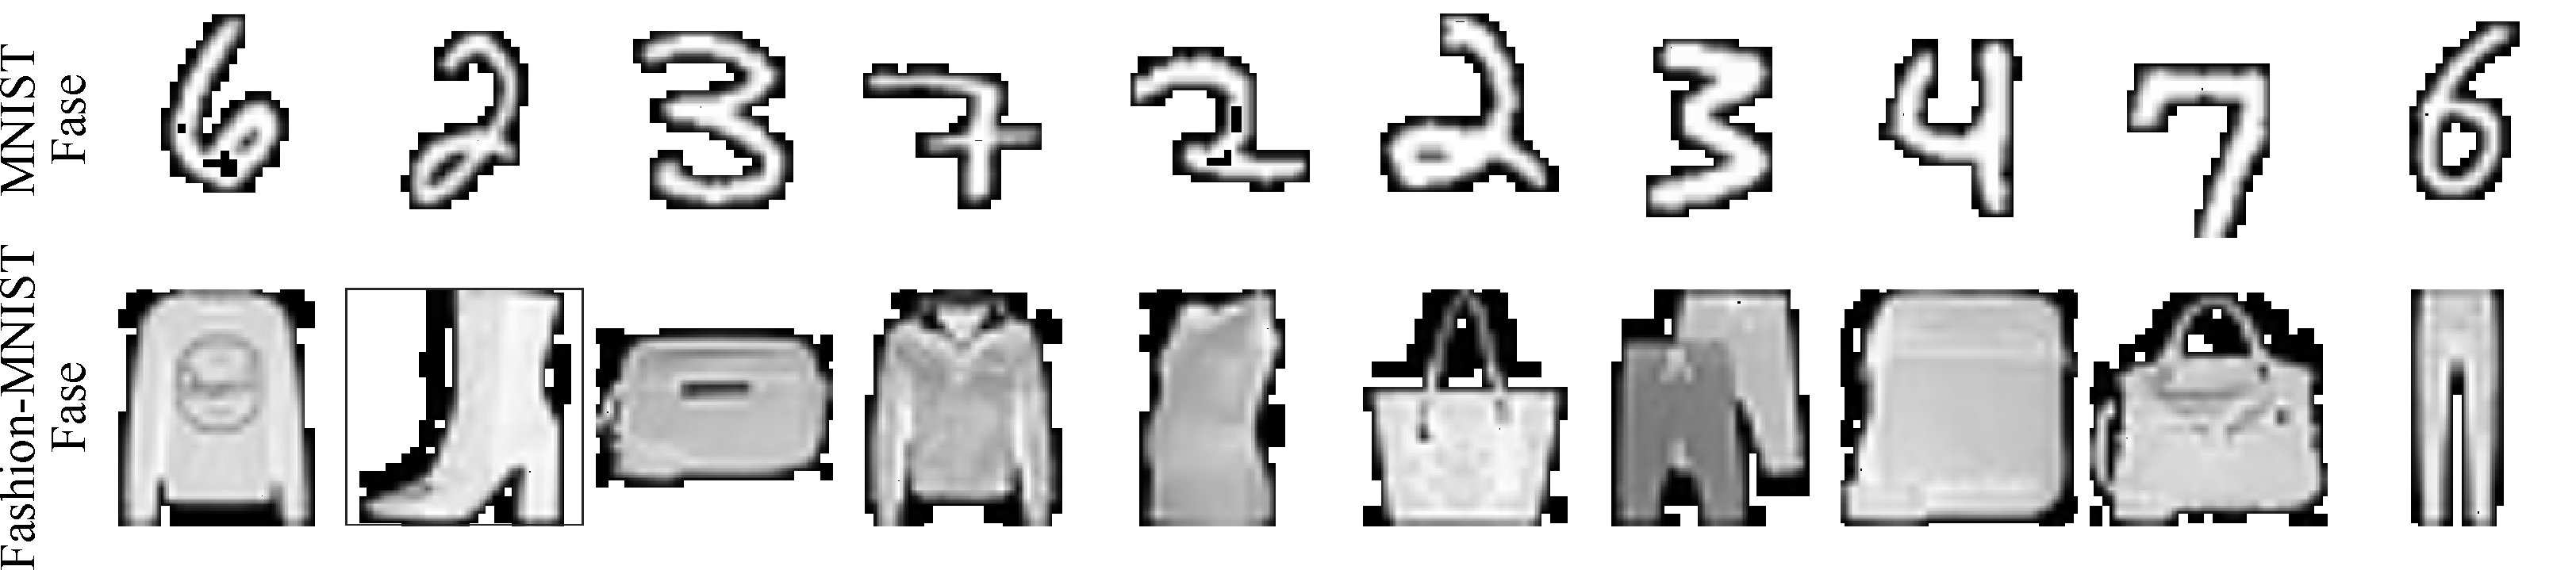
\includegraphics[width=\linewidth]{images/resultados/datasets.pdf}
    \label{fig:conjunto_datos}
\end{figure}


% Please add the following required packages to your document preamble:
% \usepackage{graphicx}
\begin{table}[!h]
\caption{Resumen de la división de los conjuntos de datos usados para evaluar el método propuesto.}
\centering\scalebox{0.9}{
\resizebox{\textwidth}{!}{%
\begin{tabular}{|c|c|c|c|c|}
\hline
\textbf{Conjunto de datos} & \textbf{Entrenamiento} & \textbf{Validación} & \textbf{Prueba} & \textbf{Total} \\ \hline
MNIST                      & 54000                  & 6000                & 10000           & 70000          \\ \hline
Fashion-MNIST              & 54000                  & 6000                & 10000           & 70000          \\ \hline
\end{tabular}%
}}
\label{tab:conjunto_datos}
\end{table}

\section{MÉTRICAS}
La calidad de la inicialización y la precisión de la clasificación en sistemas de difracción basados en medidas cuadráticas codificadas, se mide a través de las siguientes métricas.
\subsection{Métricas para evaluar la inicialización.}

A continuación, se describen las métricas usadas para evaluar la estimación inicial $\hat{\mathbf{z}}$ respecto a la imagen de referencia $\mathbf{z}$.
\begin{itemize}
    \item Medida del índice de similitud estructural (SSIM):
    
    \begin{equation}
        %\nonumber
        \mathrm{SSIM}(\mathbf{z}, \tilde{\mathbf{z}}) = \frac{2(\mu_{\mathbf{z}}\mu_{\tilde{\mathbf{z}}} + C_1) + (2\sigma_{\mathbf{z}\tilde{\mathbf{z}}} + C_2)}{(\mu_{\mathbf{z}} + \mu_{\tilde{\mathbf{z}}} + C_1)(\sigma_{\mathbf{z}}\sigma_{\tilde{\mathbf{z}}} + C_1)},
        \label{eq:SSIM}
    \end{equation}
    
    donde $(\mu_{\mathbf{z}}, \sigma_{{\mathbf{z}}})$ y $(\mu_{\tilde{\mathbf{z}}}, \sigma_{\tilde{\mathbf{z}}})$ representan la media y la varianza de ${\mathbf{z}}$ y $\tilde{\mathbf{z}}$ respectivamente, además $\sigma_{\mathbf{z}\tilde{\mathbf{z}}}$ es la covarianza entre ellos. Por último, $C_1 = (k_1L)^2$ y $C_2 = (k_2L)^2$ son dos constantes para prevenir división por cero y $k_1 = 0.01$ y $k_2 = 0.03$. Esta métrica tiene valores en el rango de $[0, 1]$, es decir, a mayor valor, mejor es la estimación.
    
    \item Relación de señal a ruido máxima (PSNR):
    \begin{equation}
        %\nonumber
        \mathrm{PSNR}(\mathbf{z}, \tilde{\mathbf{z}})=10 \cdot \log_{10}\left(\frac{\mathrm{MAX}^{2}}{\mathrm{MSE}(\mathbf{z}, \tilde{\mathbf{z}})}\right),
        \label{eq:PSNR}
    \end{equation}
    donde $\mathrm{MAX}(\cdot)$ es el rango dinámico de la imagen y $\mathrm{MSE}(\cdot)$ es el error cuadrático medio entre la imagen original y la estimación. Esta métrica tiene valores en el rango de $[0, \infty)$, es decir, a mayor valor, mejor es la estimación.
    
    \item Error cuadrático medio (MSE):
    
    \begin{equation}
        %\nonumber
        \mathrm{MSE}(\mathbf{z}, \tilde{\mathbf{z}}) = \frac{1}{n} \Vert \mathbf{z} - \tilde{\mathbf{z}}\Vert_2^2.
        \label{eq:MSE}
    \end{equation}
    
    Esta métrica tiene valores en el rango de $[0, \infty)$, es decir, a menor valor, mejor es la estimación.

    \item Error relativo (RE): 
    \begin{equation}
        %\nonumber
        \mathrm{RE}(\mathbf{z}, \tilde{\mathbf{z}}) = \frac{ \mathrm{dist}(\mathbf{z}, \hat{\mathbf{z}})}{\Vert \mathbf{z} \Vert_2}.
        \label{eq:RE}
    \end{equation}
    
    Esta métrica tiene valores en el rango de $[0, \infty)$, donde a menor valor, mejor es la estimación.
\end{itemize}
\subsection{Métricas para evaluar la clasificación.}
Las métricas usadas para evaluar la clasificación se presentan a continuación, donde los valores a calcular dependen de los verdaderos positivos $TP$, verdaderos negativos $TN$, falsos positivos $FP$, y falsos negativos $FN$, asociados a la clase de cada ejemplo del conjunto de datos.


\begin{itemize}
    \item Exactitud: esta medida corresponde a la proporción de predicciones predichas correctamente,

    \begin{equation}
        \mathrm{Exactitud}= \frac{TP+TN}{TP+TN+FP+FN}.
        \label{eq:acc}
    \end{equation}


    \item Precisión: esta medida es la proporción de ejemplos pertenecientes a una clase que fueron correctamente predichos en dicha clase,
    
        \begin{equation}
            \mathrm{Precisión} = \frac{TP}{TP+FP}.
            \label{eq:pre}
        \end{equation}
        
    \item Exhaustividad: esta medida es la proporción entre las predicciones que fueron correctamente clasificadas en una clase sobre los ejemplos que pertenecían a esa clase,
    
    \begin{equation}
        \mathrm{Exhaustividad}= \frac{TP}{TP+FN}.
        \label{eq:re}
    \end{equation}

    \item Métrica-F1: esta medida está diseñada para ponderar de manera equilibrada entre las métricas de precisión (\ref{eq:pre}) y exhaustividad (\ref{eq:re}),
    
    \begin{equation}
        \mathrm{F1} = \frac{2\cdot\mathrm{Precisión}\cdot\mathrm{Exhaustividad}}{\mathrm{Precisión}+\mathrm{Exhaustividad}}.
        \label{eq:f1}
    \end{equation}

\end{itemize}

\section{EXPERIMENTOS}

% \subsection{Métodos de Comparación}

% \begin{itemize}
%     \item Comparación estimación inicial.
    
%     Estimar el campo óptico inicial es una tarea ampliamente estudiada en el estado del arte de recuperación de la fase. Específicamente resaltan métodos tales como el propuesto \myfootcite{Morales:22}, \textit{orthogonality-promoting initialization} (OPI) \myfootcite{wang2017solving}, \textit{weighted maximal correlation initialization} (WMCI) \myfootcite{wang2018phase}, y \textit{filtered spectral initialization} (FSI) \myfootcite{jerez2020fast}. Estos métodos de estimación inicial son usados como etapa inicial por algoritmos de reconstrucción tales como TWF, TAF y RAF.
    
    
%     \item Comparación clasificación.
    
%     Para comparar el método propuesto se encontró que el esquema tradicional de clasificación sobre medidas cuadráticas se realiza como se muestra en la Figura \ref{fig:esquema_entrenamiento_tradicional}
    
%     \begin{minipage}[!h]{\linewidth}
      
%       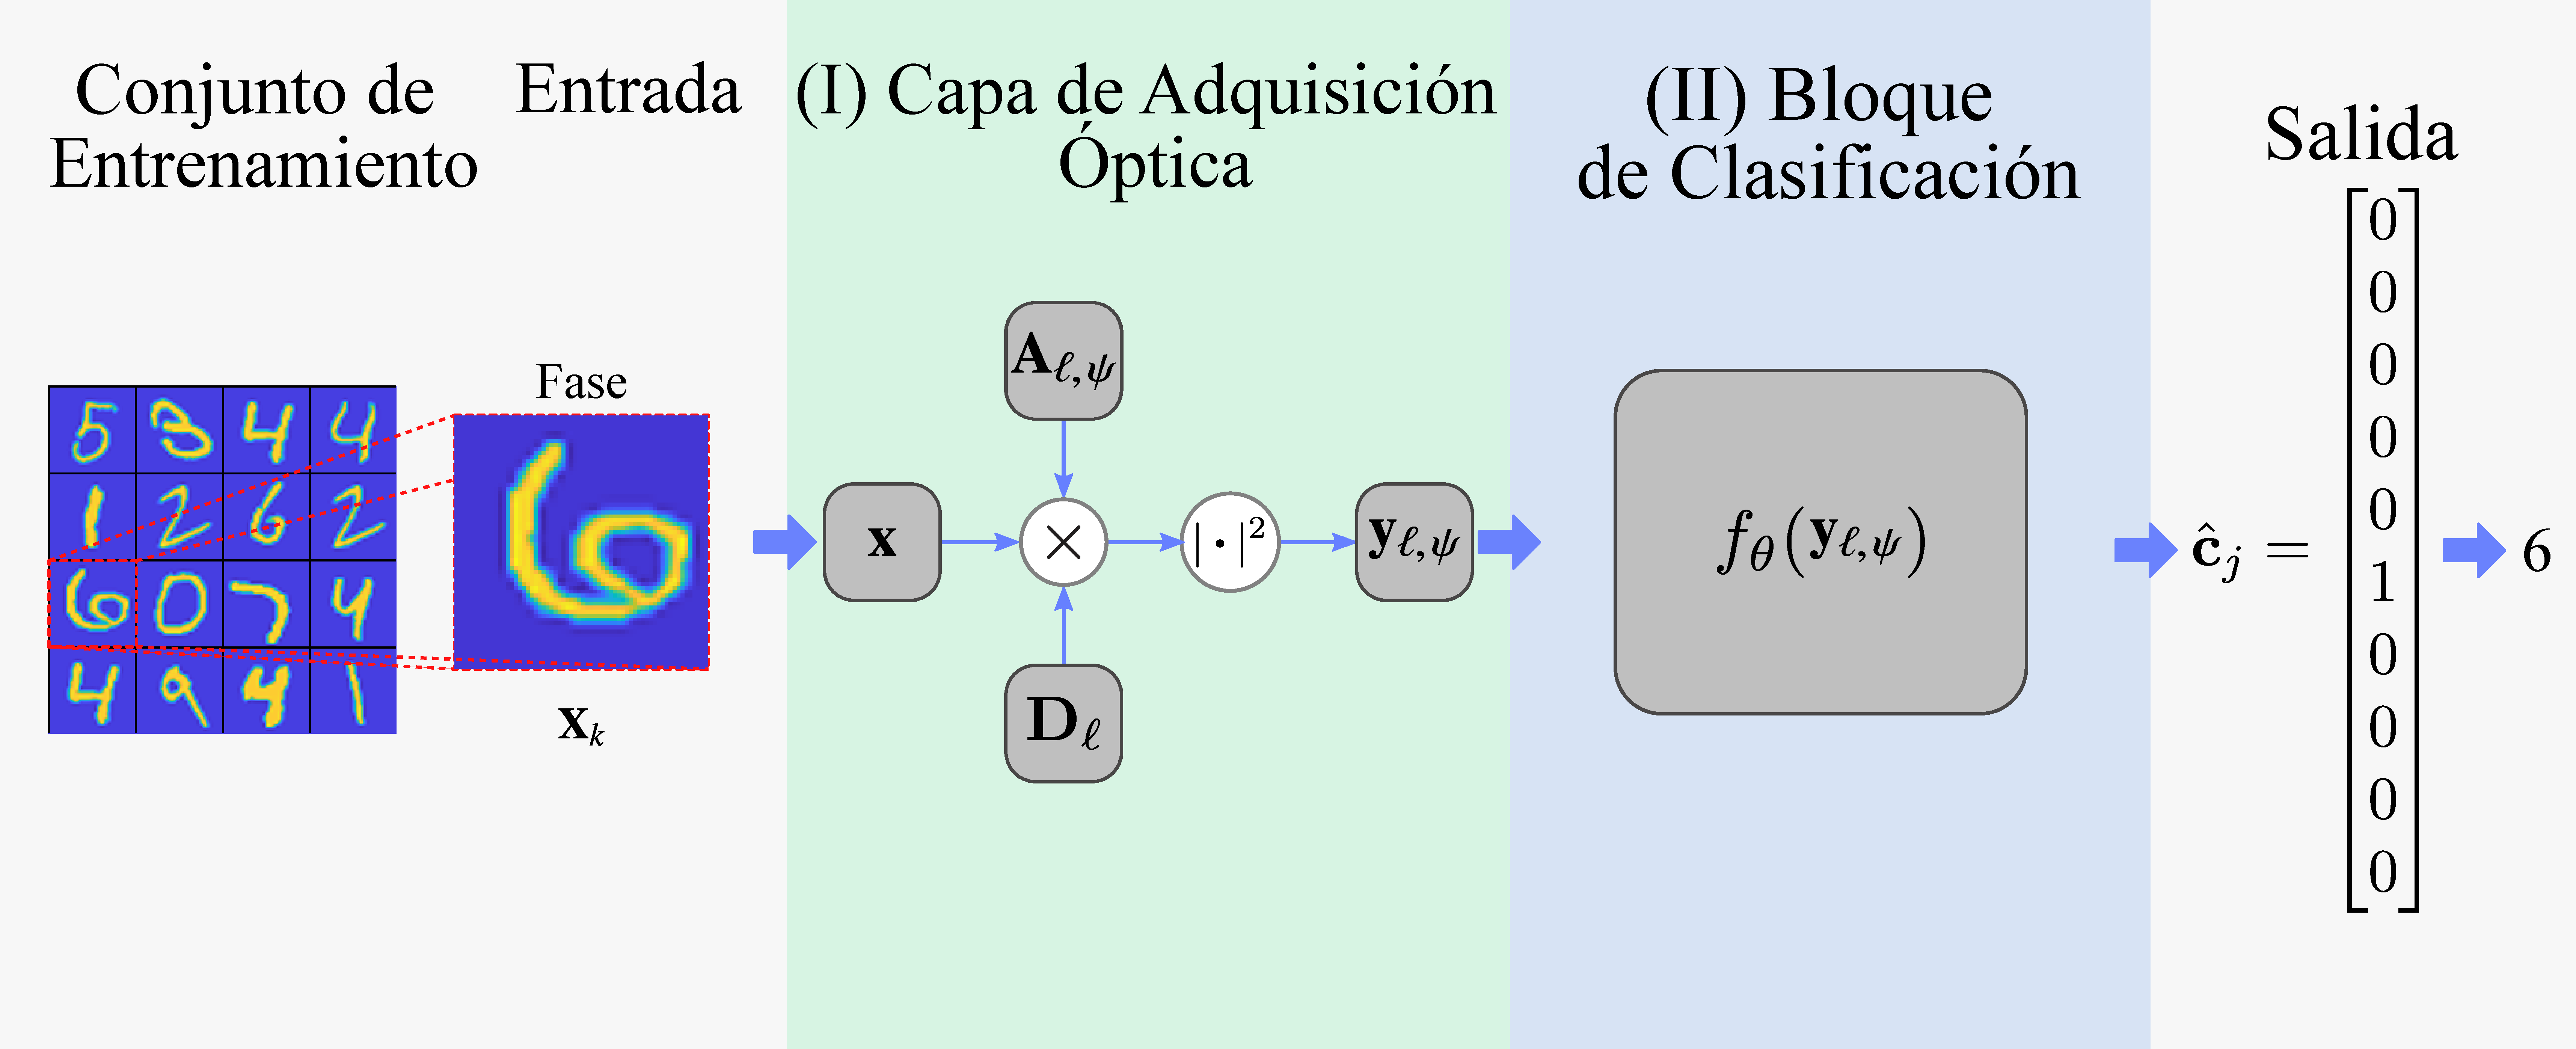
\includegraphics[width=\linewidth]{images/metodología/esquema_entrenamiento_tradicional.pdf}
%       \captionof{figure}{Esquema de clasificación usado en el estado del arte.}
%         \label{fig:esquema_entrenamiento_tradicional}
%     \end{minipage}
    
%     En el esquema tradicional no se realiza una modulación del campo óptico, por lo tanto para la comparación con el estado del arte la codificación corresponde a $\mathbf{D}_\ell = 1$.
    
%     Adicionalmente se realizó la comparación haciendo uso del operador inverso de la propagación del campo óptico $\mathcal{P}_{\ell, \psi}:\mathbb{C}^n\rightarrow \mathbb{C}^n$ para estimar $\hat{\mathbf{x}}$ \myfootcite{katkovnik2017computational},
    
%     \begin{equation}
%         \hat{\mathbf{x}}= \frac{1}{L}\sum_{\ell=1}^{ L} \mathcal{P}_{\ell, \psi}(\mathbf{y}_{\ell, \psi}).
%         \label{eq:back_propagation}
%     \end{equation}
% \end{itemize}

\subsection{Configuración experimental.}

En esta subsección, se presentan los parámetros de simulación utilizados para el modelo de propagación, la etapa de inicialización y la red neuronal de clasificación. Todos los experimentos realizados en este trabajo fueron implementados en \textit{Python 3.9} usando la herramienta \textit{Tensorflow 2.4.1}  \myfootcite{tensorflow2015-whitepaper}. Los experimentos se ejecutaron sobre un computador con GPU Nvidia 3090 RTX con 64 Gb de memoria RAM y CPU Intel(R) Xeon(R) W-3223 CPU @ 3.50GHz. El código usado para los experimentos de este trabajo puede ser consultado de manera pública en \footnote{\href{https://github.com/David-Morales-Norato/code_undergrad_thesis}{https://github.com/David-Morales-Norato/code\_undergrad\_thesis}}. En relación con los parámetros de propagación,  la Tabla \ref{tab:parameters} presenta los parámetros ópticos fijados para calcular la matriz $\mathbf{A}_{\ell,\psi}$ definida en \eqref{eq:phase_retrieval_problem} según cada campo de difracción. Estos parámetros permiten simular la adquisición de las medidas cuadráticas codificadas a lo largo de cada campo de difracción usando la capa de adquisición óptica. En la etapa de inicialización, el filtro $\mathbf{G} \in \mathbb{C}^{g\times g}$ entrenable fue fijado a un tamaño de kernel $g=5$ y un número de iteraciones $T=10$. La estimación del campo óptico inicial es una tarea ampliamente estudiada en el estado del arte de recuperación de la fase. Específicamente, se destacan métodos de inicialización, tales como \textit{orthogonality-promoting initialization} (OPI) \myfootcite{wang2017solving}, \textit{weighted maximal correlation initialization} (WMCI) \myfootcite{wang2018phase}, y FSI \myfootcite{jerez2020fast}. Cabe señalar que, estos métodos de inicialización fueron usados para comparar la inicialización propuesta LFSI, donde se comparó la robustez al ruido, el número de iteraciones ${T}$ y el número de proyecciones ${L}$ requeridas para lograr una estimación apropiada. 

Finalmente, para realizar la clasificación se usaron las arquitecturas MobilNetV2 \myfootcite{mobilnetv2}, InceptionV3 \myfootcite{inceptionv3} y Xception \myfootcite{xception}, las cuales fueron entrenadas usando una tasa de aprendizaje de $1\times 10^{-3}$ con el algoritmo de optimización Adam a partir de $\mathcal{E}=100$ épocas para entrenar los conjuntos de datos MNIST y Fashion-MNIST. Para comparar el esquema de clasificación propuesto se implementó el esquema de clasificación tradicional \myfootcite{kim2018deep}$^,$\myfootcite{ ziletti2018insightful}, donde se realiza únicamente el proceso de simulación de las medidas cuadráticas sin el proceso de estimación del campo óptico. Asimismo, se empleó el método propuesto de filtrado espectral aprendido en las Figuras \ref{fig:results_mob}, \ref{fig:results_inc} y \ref{fig:results_xce}. Por otra parte, se reemplazó en la etapa de inicialización del esquema de clasificación propuesto, el algoritmo de inicialización LFSI por el modelo de propagación inverso (BPM, de sus siglas en inglés \textit{back-propagation matrix}) $\mathbf{A}_{\ell, \psi}^{-1}$ para obtener una estimación rápida del campo óptico inicial, como se presenta en las Figuras \ref{fig:results_mob}, \ref{fig:results_inc} y  \ref{fig:results_xce}. Esta estimación rápida está dada por 

\begin{equation}
    \hat{\mathbf{z}}= \frac{1}{L}\sum_{\ell=1}^{ L} \mathbf{A}_{\ell, \psi}^{-1}\mathbf{y}_{\ell, \psi}
    \label{eq:back_propagation}.
\end{equation}

Es importante señalar que, $\mathbf{z} \neq \mathbf{A}_{\ell, \psi}^{-1}\mathbf{y}_{\ell}$, debido a la pérdida de la información de fase que induce el operador de magnitud $\vert \cdot \vert$ presente en el modelo de propagación \eqref{eq:phase_retrieval_problem}.


% Por último, todos los experimentos realizados en este trabajo fueron implementados en \textit{Python 3.9} usando la herramienta \textit{Tensorflow 2.4.1}  \myfootcite{tensorflow2015-whitepaper}. Los experimentos se ejecutaron sobre un computador con GPU Nvidia 3090 RTX con 64 Gb de memoria RAM y CPU Intel(R) Xeon(R) W-3223 CPU @ 3.50GHz. El código usado para los experimentos de este trabajo puede ser consultado de manera pública en el siguiente enlace: \href{https://github.com/David-Morales-Norato/code_undergrad_thesis}{https://github.com/David-Morales-Norato/code\_undergrad\_thesis}

\begin{table}[!h]
\centering
\caption{ Parámetros de propagación usados para simular el modelo de propagación \eqref{eq:phase_retrieval_problem} para cada campo de difracción.}
\scalebox{0.9}{
\begin{tabular}{|l|r|r|c|}
\hline
\multicolumn{1}{|c|}{\textbf{Parámetros ópticos}} & \multicolumn{1}{c|}{\textbf{Campo cercano}} & \multicolumn{1}{c|}{\textbf{Campo medio}} & \textbf{Campo lejano} \\ \hline
Longitud de onda ($\lambda$) [nm]                    & 635                           & 635                            & -         \\ \hline
Distancia de propagación ($z$) [cm]         &    2.5                       & 7                              & -         \\ \hline
\end{tabular}}
\label{tab:parameters}
\end{table}


\subsection{Resultados de la inicialización.}


La Figura \ref{fig:results_initializations} muestra el desempeño en la métrica de RE del método de estimación inicial propuesto comparando con los algoritmos FSI, OPI y WMCI variando el número de iteraciones $T$ para los conjuntos de datos MNIST y Fashion-MNIST en los tres campos de difracción cercano, medio y lejano, donde se puede observar que el método propuesto logra superar los métodos tradicionales obteniendo una estimación inicial apropiada a partir de un número menor de iteraciones.

\begin{figure}[!h]
\centering
    \caption{Resumen del desempeño de la inicialización propuesta comparando con los métodos FSI, OPI, WMCI sobre la métrica de RE, variando el número de iteraciones del algoritmo para estimar imágenes de los conjuntos MNIST y Fashion-MNIST en los campos de difracción cercano, medio y lejano.}
    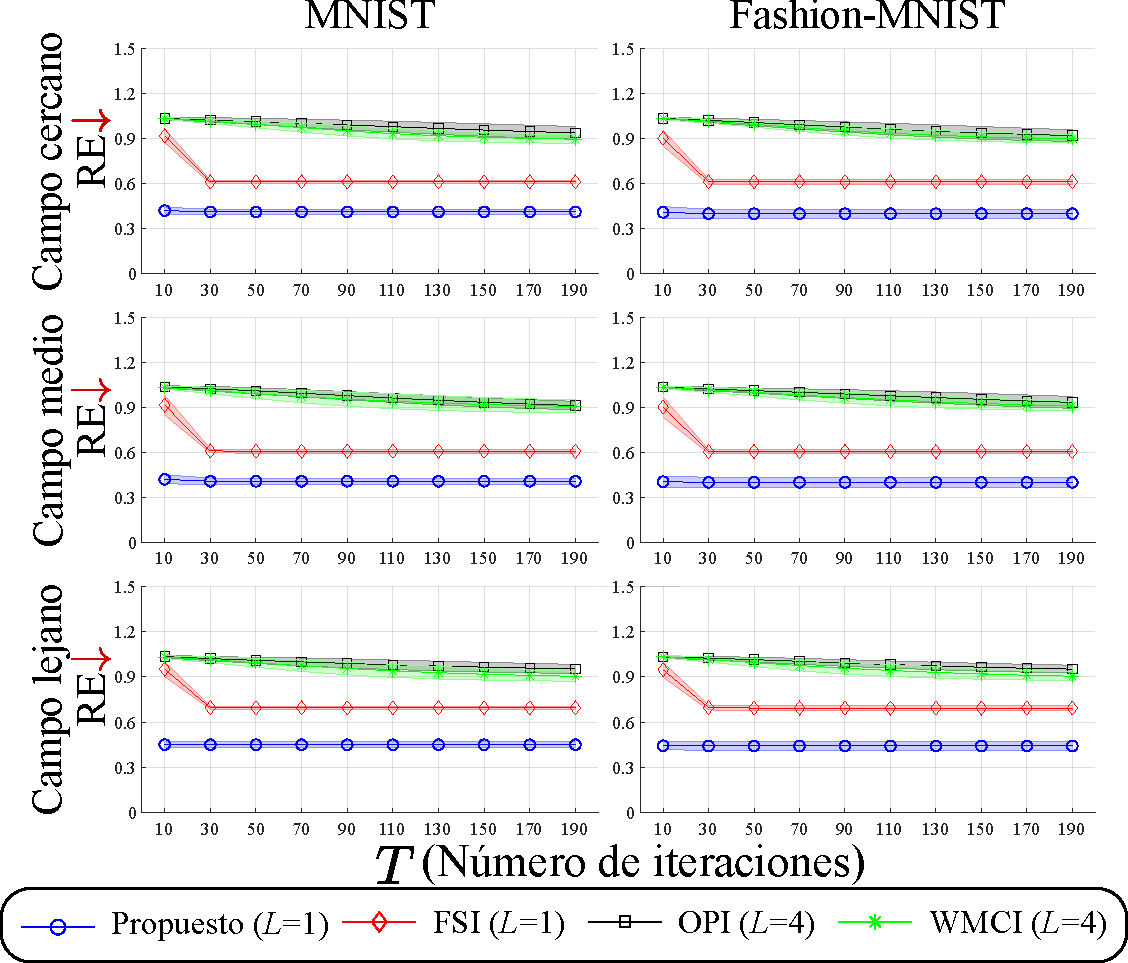
\includegraphics[width=0.85\linewidth]{images/resultados/results_initializations.pdf}
        \label{fig:results_initializations}
\end{figure}



La Figura \ref{fig:noisy_scenario} muestra la evaluación de la robustez del método frente al ruido. En este caso, se adicionó ruido aditivo gaussiano con $\mathrm{SNR} = 10, 15$ y $30$. Cabe resaltar que, el método propuesto muestra una mayor estabilidad al ruido comparando con los métodos de inicialización del estado del arte.

\begin{figure}[!h]
    \caption{Resumen del desempeño de la inicialización comparando con diferentes estrategias del estado del arte. Se varió el número de medidas $T$ para realizar la estimación y diferentes niveles de ruido afectando las medidas descritos por el SNR.}
    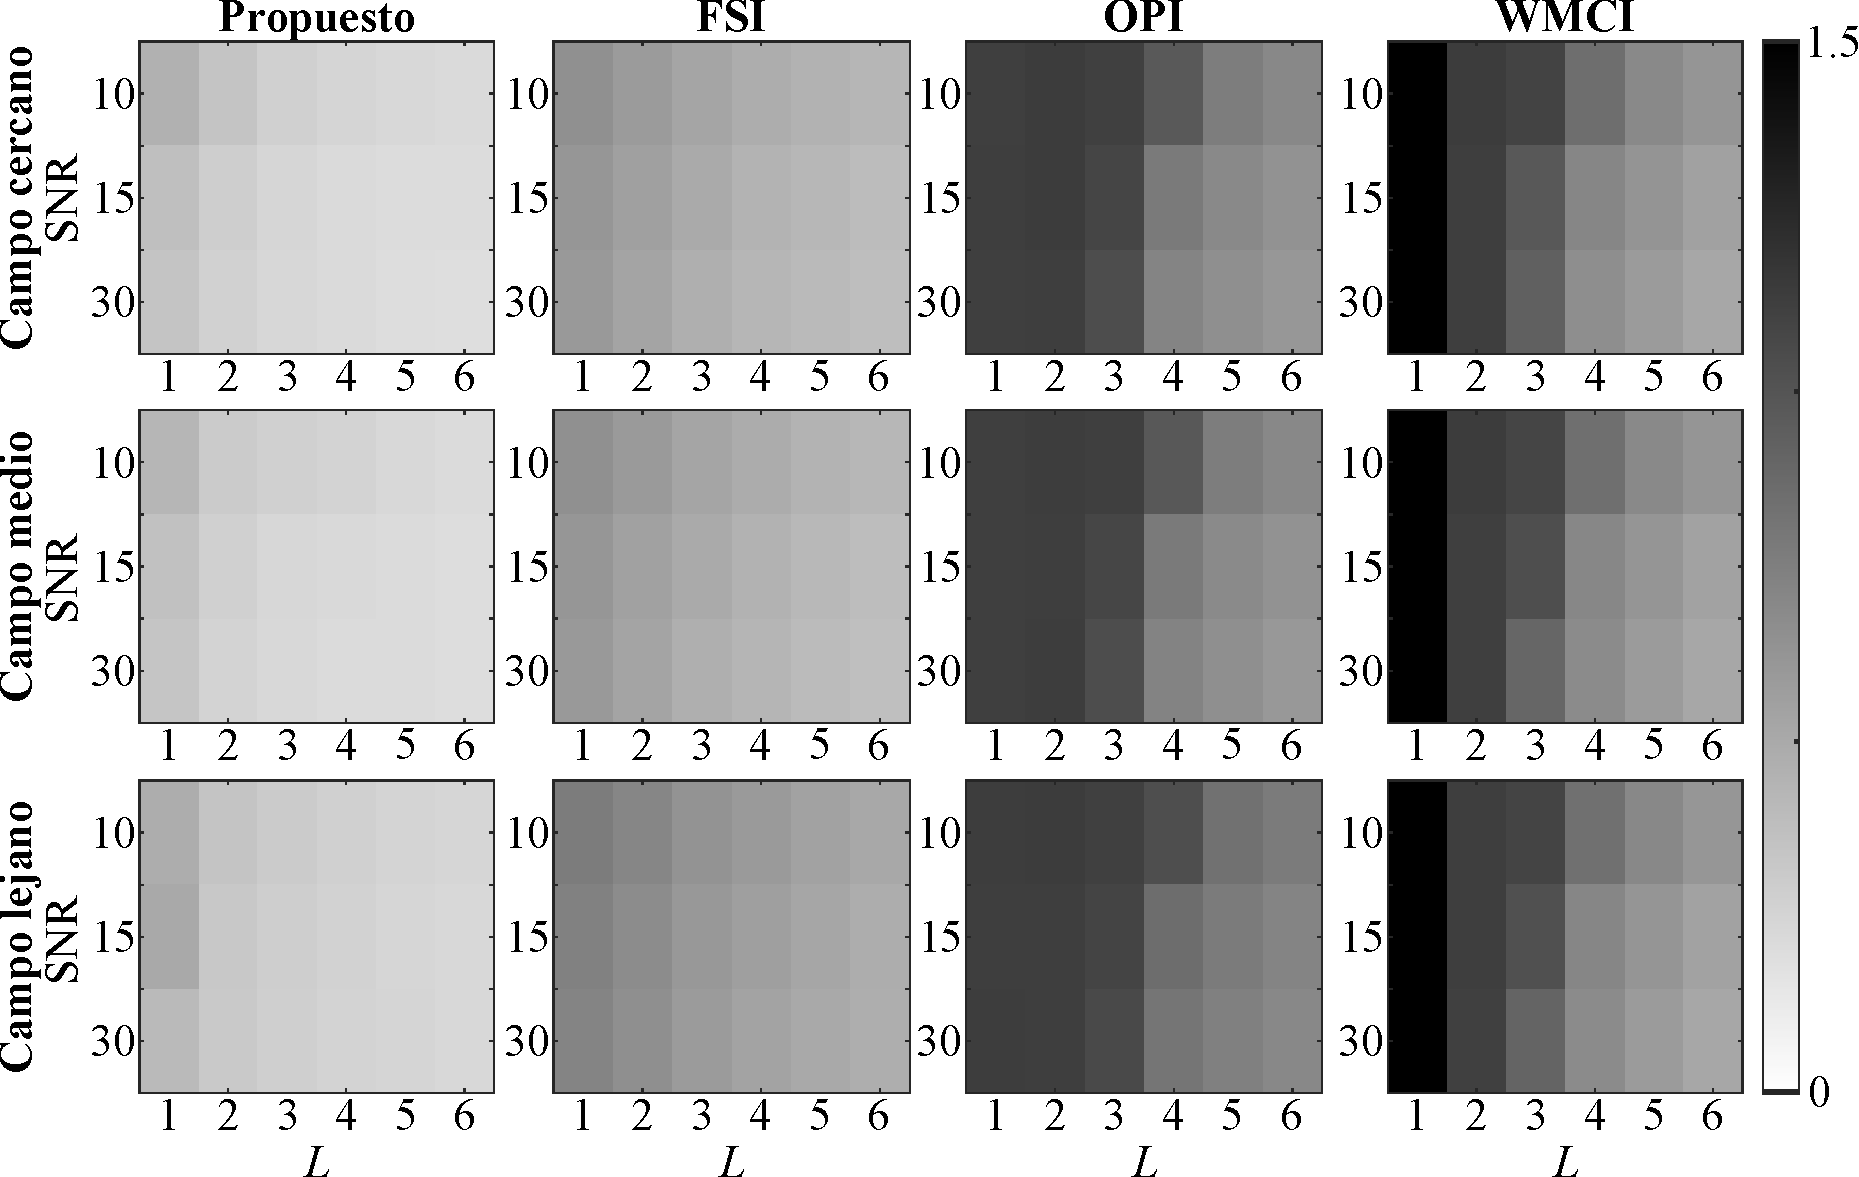
\includegraphics[width=1\linewidth]{images/resultados/Noisy_Initializations.pdf}
    \label{fig:noisy_scenario}
\end{figure}

Por último, la Figura \ref{fig:resultados_inicialización_sin_ruido} presenta los resultados visuales de la estimación del campo inicial para el conjunto de datos MNIST y Fashion-MNIST. Para comparar el método propuesto se implementaron los algoritmos FSI con $L = 1, T = 10$, FSI usando $L = 1, T=200$, OPI $L = 4, T=200$ y WMCI $L = 4, T=200$. Se puede observar que, el método propuesto logra aproximar el campo óptico en los tres campos de difracción simulados a un bajo número de iteraciones utilizando una única proyección $L=1$ y $T=10$ número de iteraciones.

\begin{figure}[!h]
    \centering
    \caption{Resultados visuales de la estimación del campo óptico inicial comparando el método propuesto contra el algoritmo FSI con $L = 1, T = 10$, FSI usando $L = 1, T=200$, OPI $L = 4, T=200$ y WMCI $L = 4, T=200$.}
    \includegraphics[width=\linewidth]{images/resultados/resultados_inicialización_sin_ruido.pdf}
    \label{fig:resultados_inicialización_sin_ruido}
\end{figure}

\pagebreak

\subsection{Resultados de la clasificación de objetos.}

Los resultados de los experimentos de clasificación se resumen a continuación. Las Figuras \ref{fig:results_mob}, \ref{fig:results_inc} y \ref{fig:results_xce} exhiben los resultados del desempeño de la clasificación de medidas cuadráticas codificadas en términos de las métricas de exactitud, precisión, exhaustividad y F1 utilizando las redes de clasificación MobilNetV2 en la Figura \ref{fig:results_mob}, InceptionV3 en la Figura \ref{fig:results_inc} y Xception en la Figura \ref{fig:results_xce}. Cada figura representa la comparación de los esquemas de clasificación tradicional, y los métodos propuestos BPM y LFSI. La clasificación se realizó sobre medidas simuladas en los campos de difracción cercano, medio y lejano. Es importante resaltar que, el método tradicional muestra un desempeño menor en todas las métricas comparando con los métodos propuestos BPM y LFSI para cada uno de los campos de difracción y redes de clasificación.

Específicamente, el método propuesto supera al método tradicional en hasta 0.24, 0.2, 0.25 y 0.22 en términos de exactitud, precisión, exhaustividad y métrica F1, respectivamente. En particular, estas ganancias se reportan para la clasificación de objetos utilizando medidas simuladas del campo lejano a partir del conjunto de datos de Fashion-MNIST. En el caso del campo medio, se supera en 0.21, 0.13, 0.21, y 0.17 y para el campo cercano, se supera en 0.1, 0.14, 0.13, y 0.14 en exactitud, en precisión, en exhaustividad y en F1, respectivamente. 

\begin{figure}[!h]
    \centering
    \caption{Resultados en la métrica de exactitud, precisión, exhaustividad y F1 para evaluar la clasificación de medidas cuadráticas codificadas simuladas sobre el campo cercano, medio y lejano. Se muestra la comparación de la clasificación Tradicional, el uso del propagador inverso propuesto (BPM) y el método de inicialización aprendida (LFSI) usando la arquitectura MobilNetV2, sobre la división de prueba de los conjuntos de datos MNIST y Fashion-MNIST.}
    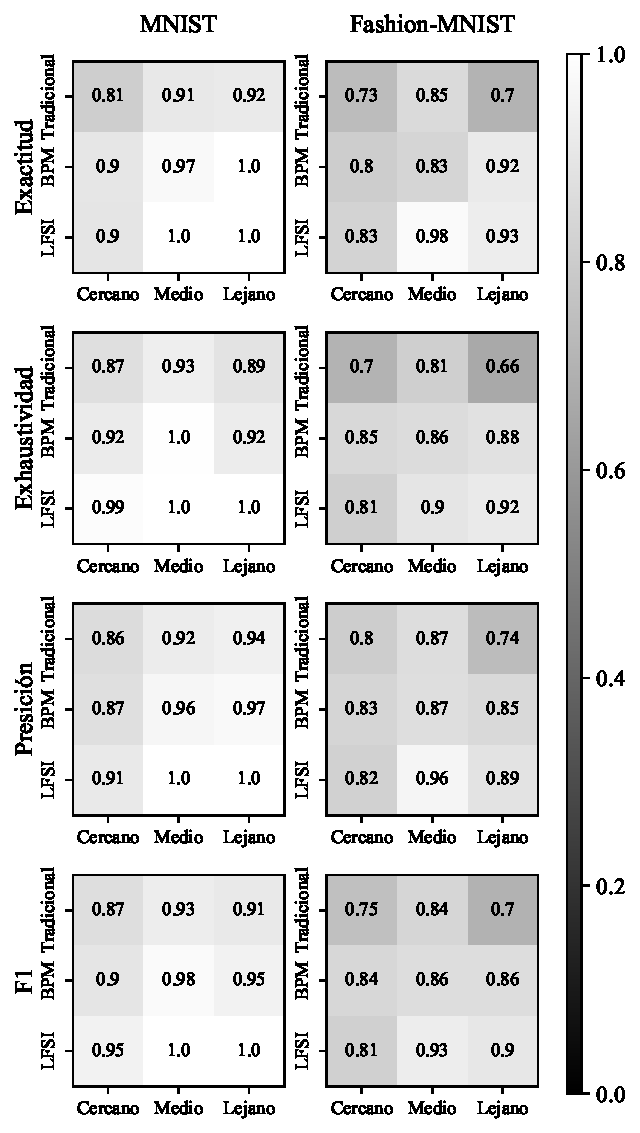
\includegraphics[height=0.8\textheight]{images/resultados/test_result_mobilnet.pdf}
    \label{fig:results_mob}
\end{figure}


\begin{figure}[!h]
    \centering
    \caption{Resultados en la métrica de exactitud, precisión, exhaustividad y F1 para evaluar la clasificación de medidas cuadráticas codificadas simuladas sobre el campo cercano, medio y lejano. Se muestra la comparación de la clasificación Tradicional, el uso del propagador inverso propuesto (BPM) y el método de inicialización aprendida (LFSI) usando la arquitectura InveptionV3, sobre la división de prueba de los conjuntos de datos MNIST y Fashion-MNIST.}
    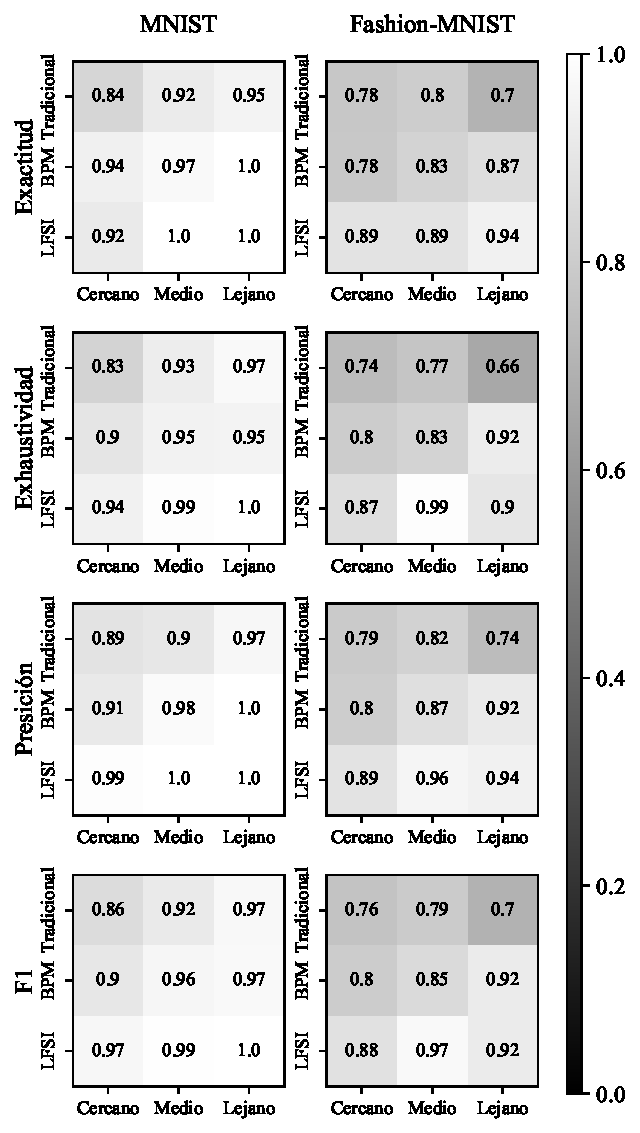
\includegraphics[height=0.8\textheight]{images/resultados/test_result_inception.pdf}
    \label{fig:results_inc}
\end{figure}

\begin{figure}[!h]
    \centering
    \caption{Resultados en la métrica de exactitud, precisión, exhaustividad y F1 para evaluar la clasificación de medidas cuadráticas codificadas simuladas sobre el campo cercano, medio y lejano. Se muestra la comparación de la clasificación Tradicional, el uso del propagador inverso propuesto (BPM) y el método de inicialización aprendida (LFSI) usando la arquitectura Xception, sobre la división de prueba de los conjuntos de datos MNIST y Fashion-MNIST.}
    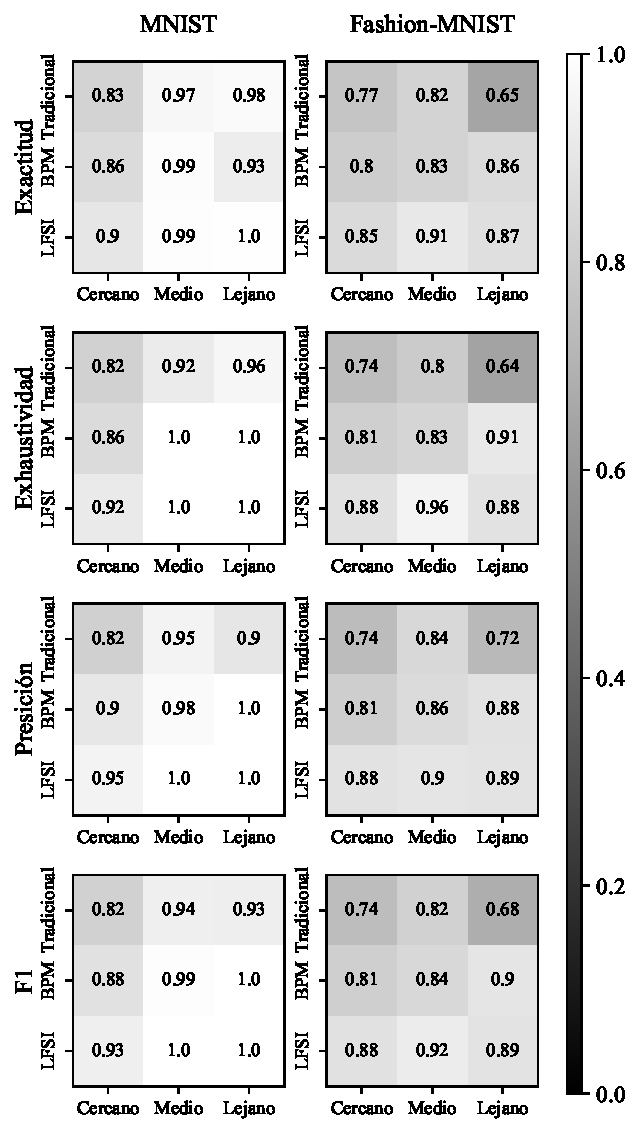
\includegraphics[height=0.8\textheight]{images/resultados/test_result_xception.pdf}
    \label{fig:results_xce}
\end{figure}
 % Controladores PI y su conjunto estabilizante
% \input{Secs/T5} % Recomendaciones
% ------------------------------------------------------------------------
% ------------------------------------------------------------------------
% ------------------------------------------------------------------------
%                            Trabajo futuro
% ------------------------------------------------------------------------
% ------------------------------------------------------------------------
% ------------------------------------------------------------------------

\chapter{TRABAJO FUTURO}
% ------------------------------------------------------------------------
% \noindent Actividades complementarias a los desarrollos presentados, incluyen el cálculo automático para conjuntos estabilizantes en plantas arbitrarias empleando el \emph{método de la signatura} desarrollado por Keel y Bhattacharyya en \myfootcite{keel2008}.\\

% Asimismo es importante explorar otras topologias de compensador y controladores PID, en sus versiones de tiempo continuo y discreto.
% ------------------------------------------------------------------------ % Trabajo futuro
% ------------------------------------------------------------------------
% ------------------------------------------------------------------------
% ------------------------------------------------------------------------
%                             Conclusiones
% ------------------------------------------------------------------------
% ------------------------------------------------------------------------
% ------------------------------------------------------------------------

\chapter{CONCLUSIONES}


En este trabajo se propuso un esquema de tres etapas para la clasificación de medidas cuadráticas codificadas utilizando aprendizaje profundo. Primero, una capa simula el proceso de adquisición. Esta capa contiene un modelo de propagación del campo óptico codificado siguiendo tres diferentes campos de difracción. Luego, un procedimiento de inicialización aproxima el campo óptico inicial mediante el desenvolvimiento de un algoritmo tradicional y el aprendizaje de un kernel convolucional. Por último, la red de clasificación infiere la clase correspondiente a cada medida cuadrática codificada según la estimación inicial. Para validar el método propuesto se realizaron experimentos sobre diferentes campos de difracción y redes de clasificación del estado del arte, tales como MobilNetV2, InceptionV3 y Xception. Adicionalmente, se emplearon los conjuntos de datos MNIST y Fashion-MNIST para evaluar los diferentes esquemas de aprendizaje profundo.

Los experimentos realizados exhiben un mejor rendimiento de clasificación usando el método propuesto comparado con el enfoque de clasificación tradicional que evalúa directamente las medidas adquiridas sin tener en cuenta el modelo físico. En particular, el método propuesto supera al método tradicional en hasta 0.24, 0.2, 0.25 y 0.22 en términos de exactitud, precisión, exhaustividad y métrica F1, respectivamente. Estas ganancias se reportan para la clasificación de objetos utilizando medidas simuladas del campo lejano a partir del conjunto de datos de Fashion-MNIST. % Conclusiones
% ------------------------------------------------------------------------
% Bibliografía
% ------------------------------------------------------------------------
\printbibliography[heading=bibintoc,title={BIBLIOGRAFÍA},omitnumbers=true]
% ------------------------------------------------------------------------
% Anexos
% ------------------------------------------------------------------------
% % ------------------------------------------------------------------------
% ------------------------------------------------------------------------
% ------------------------------------------------------------------------
%                                Anexo A
% ------------------------------------------------------------------------
% ------------------------------------------------------------------------
% ------------------------------------------------------------------------
% ------------------------------------------------------------------------
\nnchapter{ANEXOS}
% ------------------------------------------------------------------------
\anexo{Fundamentos de sólidos rígidos}\label{anexoA}
% ------------------------------------------------------------------------
Un sólido rígido, es un cuerpo formado por varias partículas puntuales que
guardan distancias constantes entre sí \myfootcite{sears2005fisica}.\\

Una operación fundamental para definir cantidades en el espacio de movimiento de
un sólido rígido es el producto vectorial (también denominado producto cruz \myfootcite{stanley1993algebra}),
el cual produce un vector perpendicular (normal) al plano formado por otros dos vectores
que se multiplican.\\

Sean dos vectores $\vec{a}$ y $\vec{b}$ definidos en $\mathbb{R}^3$. El producto vectorial entre $\vec{a}$ y $\vec{b}$ (denotado $\vec{a} \times \vec{b}$) es otro vector (digamos $\vec{c} \in \mathbb{R}^3$) cuyo cálculo puede ser efectuado a través de determinantes como sigue:
% ------------------------------------------------------------------------
\begin{equation}\label{defprodvect}
\vec{c} = \vec{a} \times \vec{b} = \begin{vmatrix}
i& j & k \\
a_i & a_j  & a_k \\
b_i & b_j  & b_k
\end{vmatrix} =
\begin{vmatrix}
 a_j & a_k \\
 b_j & b_k
\end{vmatrix}i~
-
\begin{vmatrix}
a_i & a_k \\
b_i & b_k
\end{vmatrix}j~
+\begin{vmatrix}
 a_i & a_j \\
 b_i & b_j
\end{vmatrix}k
\end{equation}
% ------------------------------------------------------------------------
De esta manera, siendo $\vec{a}=(1,-1,2)$ y $\vec{b}=(3,-4,5)$ se obtiene:
% ------------------------------------------------------------------------
\begin{equation}
\vec{a} \times \vec{b} =\begin{vmatrix}
i& j & k \\
1 &-1  &2 \\
3 &-4  &5
\end{vmatrix}=
\begin{vmatrix}
 -1&2 \\
 -4&5
\end{vmatrix}i~
-
\begin{vmatrix}
1 &2 \\
3 &5
\end{vmatrix}j~
+\begin{vmatrix}
 1&-1 \\
 3&4
\end{vmatrix}k
= 3i-j-k
\end{equation}
% ------------------------------------------------------------------------
\noindent La Fig. \ref{prodvect} ilustra esta operación gráficamente en el espacio tridimensional.
% ------------------------------------------------------------------------
\begin{figure}[h]
\centering
\caption[]{Ilustración gráfica para producto vectorial}\label{prodvect}
\includegraphics[width=0.3\textwidth]{Figs/prodvect}
% Si la figura posee una fuente distinta a los autores descomente la línea a continuación de este comentario,
% tomando en cuenta que debe realizar una cita previa fuera del caption para crear la referencia, tal y como
% lo presenta el ejemplo para la Figura \label{cuerpolibre}
% \caption*{Fuente: \arabic{footnote}.}
\end{figure}
% ------------------------------------------------------------------------

\section*{Condición de rigidez}
% ------------------------------------------------------------------------
Considere el sólido rígido presentado en la Fig. \ref{rigid}. Para cada pareja de puntos $(P_i, P_j)$ pertenecientes al sólido, se cumple:
% ------------------------------------------------------------------------
\begin{equation}\label{rigidez}
\frac{d}{dt}[\left|r_i - r_j\right|] = \frac{d}{dt}[\left|r_{ij}\right|] = 0,
\end{equation}
% ------------------------------------------------------------------------
lo cual significa que la distancia entre puntos de un sólido rígido se mantiene invariante. Esto último se conoce como la \emph{condición de rígidez}.\\
% ------------------------------------------------------------------------
\begin{figure}[h]
\centering
\caption[]{Sólido rígido}\label{rigid}
\includegraphics[width=0.3\textwidth]{Figs/rigid}
% Si la figura posee una fuente distinta a los autores descomente la línea a continuación de este comentario,
% tomando en cuenta que debe realizar una cita previa fuera del caption para crear la referencia, tal y como
% lo presenta el ejemplo para la Figura \label{cuerpolibre}
% \caption*{Fuente: \arabic{footnote}.}
\end{figure}
% ------------------------------------------------------------------------

\noindent Asimismo, a partir de \eqref{rigidez} se obtiene:
% ------------------------------------------------------------------------
\begin{equation}
\frac{d}{dt}[\left|r_i - r_j\right|] = \left|\dot{r}_i - \dot{r}_j\right| = 0,
\end{equation}
% ------------------------------------------------------------------------
y por tanto, sabiendo que $\vec{\dot{r}}$ es el vector velocidad $\vec{v}$ para un punto del sólido visto desde el observador, es posible escribir:
% ------------------------------------------------------------------------
\begin{equation}
\left|v_i\right| = \left|v_j\right|,
\end{equation}
% ------------------------------------------------------------------------
con lo cual la velocidad de traslación para cualquier punto del sólido será la misma, y así, una vez definido el movimiento de un punto cualquiera del cuerpo rigido que se traslada en el espacio, es posible definir la totalidad de su movimiento.

% ------------------------------------------------------------------------
\section*{Movimiento de rotación}
% ------------------------------------------------------------------------
En la Fig. \ref{rotacion} se ilustra un punto que rota alrededor de un eje fijo, localizado en el cuerpo del sólido.\\
% ------------------------------------------------------------------------
\begin{figure}[h]
\centering
\caption[]{Rotación de un punto del sólido alrededor de un eje fijo}\label{rotacion}
\includegraphics[width=0.3\textwidth]{Figs/rotacion}
% Si la figura posee una fuente distinta a los autores descomente la línea a continuación de este comentario,
% tomando en cuenta que debe realizar una cita previa fuera del caption para crear la referencia, tal y como
% lo presenta el ejemplo para la Figura \label{cuerpolibre}
% \caption*{Fuente: \arabic{footnote}.}
\end{figure}
% ------------------------------------------------------------------------

\noindent A partir de ello, es posible definir la velocidad angular que experimenta el punto $P$ alrededor del eje de rotación, en el modo siguiente:
% ------------------------------------------------------------------------
\begin{equation}
\omega = \frac{d}{dt}\theta
\end{equation}\
% ------------------------------------------------------------------------

\noindent Tambien, puede escribirse del diagrama la velocidad tangencial $v$ del punto mediante:
% ------------------------------------------------------------------------
\begin{equation}
\vec{v} = \vec{r} \times \vec{\omega},
\end{equation}
% ------------------------------------------------------------------------
siendo $\vec{r}$ el vector que marca la distancia del punto $P$ al eje de rotación $O$.\\

\noindent Por tanto, el vector de aceleración puede ser formulado como:
% ------------------------------------------------------------------------
\begin{eqnarray}\label{aceler}
\nonumber \frac{d}{dt}\vec{v} & = & \frac{d}{dt}[\vec{r} \times \vec{\omega}]\\
\nonumber & = & \left( \frac{d}{dt}\vec{r}\times \vec{\omega}\right) + \left( \vec{r}\times \frac{d}{dt}\vec{\omega}\right)\\
\vec{a}   & = & \vec{r} \times \vec{\alpha},
\end{eqnarray}
% ------------------------------------------------------------------------
con $\vec{a}$ y $\vec{\alpha}$ representando, respectivamente, los vectores de aceleración lineal y angular. Note que se asume $\frac{d}{dt}\vec{r} = 0$ debido a que el eje de rotación es fijo.

% ------------------------------------------------------------------------
\section*{Conservación del momento angular}
% ------------------------------------------------------------------------
\noindent En un movimiento traslacional, el principio de conservación del momento lineal establece:
% ------------------------------------------------------------------------
\begin{equation}
\frac{d}{dt}\vec{p} = \frac{d}{dt}{m\vec{v}} = 0,
\end{equation}
% ------------------------------------------------------------------------
a partir de lo cual el momento $\vec{p}$ será constante en ausencia de fuerzas externas.\\

De manera similar, es posible definir el momento angular $\vec{\mathbf{L}}$ de una partícula de masa puntual que rota alrededor de un eje fijo, en el modo siguiente:
% ------------------------------------------------------------------------
\begin{equation}\label{momang}
\vec{\mathbf{L}} = \vec{r} \times \vec{p},
\end{equation}
% ------------------------------------------------------------------------
siendo $\vec{r}$ el vector de distancia a la masa desde el centro de rotación.\\

\noindent Por tanto, el principio de conservación del momento angular puede establecerse como sigue:
% ------------------------------------------------------------------------
\begin{eqnarray*}
\frac{d}{dt}\vec{\mathbf{L}} & = & \frac{d}{dt}{[\vec{r} \times \vec{p}]} \\
                             & = & \frac{d}{dt}{[\vec{r} \times m\vec{v}]}\\
                             & = & m \frac{d}{dt}{[\vec{r} \times \vec{v}]}\\
                             & = & m\left([\vec{r}\times\frac{d}{dt}\vec{v}]+[\frac{d}{dt}\vec{r}\times\vec{v}]\right)\\
                             & = & m\left([\vec{r}\times \vec{a}]+[\vec{v}\times\vec{v}]\right)\\
                             & = & \vec{r}\times m\vec{a}\\
                             & = & \vec{r}\times \vec{F}\\
                             & = & \tau,
\end{eqnarray*}
% ------------------------------------------------------------------------
siendo $\tau$ el torque neto aplicado.\\

\noindent Empleando \eqref{aceler} puede relacionarse este torque con la aceleración angular $\vec{\alpha}$, a partir de:
% ------------------------------------------------------------------------
\begin{eqnarray*}
\tau & = & \vec{r}\times m\vec{a}\\
     & = & \vec{r}\times m\left(\vec{r} \times \vec{\alpha}\right)\\
     & = & m\left(\vec{r}\times \left(\vec{r} \times \vec{\alpha}\right)\right)
\end{eqnarray*}
% ------------------------------------------------------------------------
donde, si $\vec{r}$ es perpendicular a $\vec{\alpha}$, entonces el producto vectorial se reduce al producto de las magnitudes:
% ------------------------------------------------------------------------
\begin{eqnarray}\label{newrot}
\nonumber \tau & = & m r^2 \alpha \\
               & = & I \alpha,
\end{eqnarray}
% ------------------------------------------------------------------------
siendo $I$ el momento de inercia de las partes rotativas del cuerpo rígido.\\

\noindent La expresión \eqref{newrot} es la segunda ley de Newton de rotación, y podrá ser definida siempre que sea válido un $I$ constante. Dicha situación no siempre es posible, principalmente si se asume que el eje de rotación puede variar en el tiempo. En tal caso, $\vec{r}$ en la Fig. \ref{rotacion} no es constante y por tanto no es válida la solución propuesta para $\vec{a}$ en \eqref{aceler}, resultando en la siguiente definición alternativa para $\tau$:
% ------------------------------------------------------------------------
\begin{eqnarray*}
\tau & = & \vec{r}\times m\vec{a}\\
     & = & \vec{r}\times m\left(\left( \frac{d}{dt}\vec{r}\times \vec{\omega}\right) + \left( \vec{r}\times \frac{d}{dt}\vec{\omega}\right)\right)\\
     & = & m\left(\left[\vec{r}\times\left( \frac{d}{dt}\vec{r}\times \vec{\omega}\right)\right] + \left[\vec{r}\times\left( \vec{r}\times \vec{\alpha}\right)\right]\right)\\
     & = & m\left(\left[\vec{r}\times\left( \frac{d}{dt}\vec{r}\times \vec{\omega}\right)\right]\right) + I\alpha.
\end{eqnarray*}\
% ------------------------------------------------------------------------

\noindent El término
% ------------------------------------------------------------------------
$$
m\left(\left[\vec{r}\times\left( \frac{d}{dt}\vec{r}\times \vec{\omega}\right)\right]\right),
$$\
% ------------------------------------------------------------------------

\noindent representa los efectos (torques) debidos a las variaciones del eje de rotación, que evidentemente también representan variaciones del vector de momento angular $\vec{\mathbf{L}}$. Dichos efectos se denominan \emph{fuerzas inerciales}, puesto que tienen sentido en un marco de referencia de un cuerpo en rotación. Los tipos más representativos de fuerza inercial son los efectos giroscópicos y la fuerza de Coriollis \myfootcite{sears2005fisica}.
% ------------------------------------------------------------------------  % Fundamentos de sólidos rígidos
% % ------------------------------------------------------------------------
% ------------------------------------------------------------------------
% ------------------------------------------------------------------------
%                                Anexo B
% ------------------------------------------------------------------------
% ------------------------------------------------------------------------
% ------------------------------------------------------------------------
% ------------------------------------------------------------------------
\newpage
\anexo{Función \emph{ode45} de MATLAB}\label{anexoB}
% ------------------------------------------------------------------------
La función $ode45$ está basada en un algoritmo de tipo Runge-Kutta, que se desarrolló a partir del método de Euler mejorado \myfootcite{chapra2003metodos}. La función recibe tres parámetros esenciales: $f(t)$ dentro de un $script$ en el que se define la ecuación diferencial acompañado por un simbolo $@$, el vector de límites de tiempo $\left[ t_0 \quad t_f \right]$ y el vector de condiciones iniciales $y_0$. En otras palabras el prototipo básico para usar \emph{ode45} es el siguiente:
% ------------------------------------------------------------------------
\begin{equation}\label{defode}
   [t,y]=\emph{ode45}(@f(t),\left[ t_0 \quad t_f \right],y_0);
    \end{equation}
% ------------------------------------------------------------------------
En este caso la solución numérica se almacenará en el vector $y$  para cada uno de los instantes de tiempo presentes en el vector $t$.\\

La función $ode45$, resuelve ecuaciones del tipo $\dot{y} = f(t,y)$, por tanto si se desea resolver ecuaciones de orden superior estas deben escribirse como un sistema de ecuaciones diferenciales de primer orden.\\

A manera de ejemplo, se ilustrará la forma de resolver la ecuación diferencial de segundo orden
% ------------------------------------------------------------------------
\begin{equation}\label{segundo}
   \ddot{x}-\mu\left(1-x^2\right)\dot{x}+x=0,
\end{equation}
% ------------------------------------------------------------------------
donde $\mu > 0$ es un parámetro escalar.\\

\noindent Por tanto, definiendo
% ------------------------------------------------------------------------

$$y_1 = x; \quad y_2 = \dot{x}$$
% ------------------------------------------------------------------------

\noindent la expresión \eqref{segundo} puede ser reescrita como
% ------------------------------------------------------------------------

$$
\dot{y}_2 = \mu \left( 1 - y_1^2 \right) y_2 + y_1
$$
% ------------------------------------------------------------------------

\noindent es decir, transformando la ecuación diferencial original de segundo orden y una variable, en una ecuación diferencial equivalente de primer orden y dos variables. Así entonces, es posible construir el vector
% ------------------------------------------------------------------------

$$
y = \left[ {\begin{array}{*{20}c}
   y_1  \\
   y_2  \\
\end{array}} \right]
$$
% ------------------------------------------------------------------------

\noindent cuya dinámica viene representada por
% ------------------------------------------------------------------------

$$
\dot{y} = \left[ {\begin{array}{*{20}c}
   f_1 \left(t, y \right)  \\
   f_2 \left(t, y \right) \\
\end{array}} \right]
$$
% ------------------------------------------------------------------------

\noindent siendo
% ------------------------------------------------------------------------

$$f_1\left(t, y \right) = y_2; \quad f_2\left(t, y \right) =  \mu \left( 1 - y_1^2 \right) y_2 + y_1$$
% ------------------------------------------------------------------------

De esta manera, evaluar la expresión \eqref{defode} permite obtener una matriz de salida $y$ con filas representando los vectores solución para $y_1$ e $y_2$ como función de $t$.\\
% ------------------------------------------------------------------------

\begin{figure}[h]
\centering
\caption[]{Diagrama de flujo para algoritmo de integración numérica de la función $ode45$ de MATLAB}\label{flujodiag}
\includegraphics[width=0.55\textwidth]{Figs/flujodiag}
% Si la figura posee una fuente distinta a los autores descomente la línea a continuación de este comentario,
% tomando en cuenta que debe realizar una cita previa fuera del caption para crear la referencia, tal y como
% lo presenta el ejemplo para la Figura \label{cuerpolibre}
% \caption*{Fuente: \arabic{footnote}.}
\end{figure}
% ------------------------------------------------------------------------

En la Fig. \ref {flujodiag} se ilustra el diagrama de flujo del algoritmo empleado para hallar la solución de una ecuación diferencial mediante integración numérica empleando la función $ode45$ de MATLAB.\\

\noindent Inicialmente, se deben asignar los parámetros definidos en la ecuación \eqref{defode}.\\

\noindent Posteriormente, un bucle interno hace llamado iterativo a la función $f(t)$ evaluada para valores de tiempo entre $t_0$ y $t_f$ a partir de las condiciones iniciales $y_0$. Para cada ciclo la condición inicial se recalcula siendo la condición final del ciclo anterior. El tiempo se incrementa en un tamaño de paso $\delta t$ de forma adaptativa, si no se especifica lo contrario. Tras alcanzarse el tiempo final $t_f$, el bucle interno termina y entrega como resultado el vector de puntos de la trayectoria solución $y(t)$ al igual que el vector de tiempos $t$.  % Función ode45 de MATLAB
% % ------------------------------------------------------------------------
% ------------------------------------------------------------------------
% ------------------------------------------------------------------------
%                                Anexo C
% ------------------------------------------------------------------------
% ------------------------------------------------------------------------
% ------------------------------------------------------------------------
% ------------------------------------------------------------------------
\newpage
\anexo{Interfaz de animación de la dinámica del sistema}\label{anexoC}
% ------------------------------------------------------------------------
En ausencia de un prototipo real para verificar el comportamiento dinámico del sistema controlado, se optó por construir una animación que permitiera recrear el movimiento del \emph{dron} de una manera cercana al comportamiento físico real. A continuación se presentan las etapas importantes para este desarrollo.

% ------------------------------------------------------------------------
\section*{Descripción general de requerimientos}
% ------------------------------------------------------------------------
Se requiere construir una interfaz de software que permita visualizar el comportamiento del dron en el espacio de movimiento, como aproximación a la operación real del sistema para diferentes condiciones de simulación (lazo abierto, lazo cerrado controlado PID y por realimentación de estados) ante la presencia de perturbaciones. La interfaz deberá permitir modificar parámetros del sistema y los parámetros de simulación, así como también entregar información de las trayectorias de variables con respecto al tiempo.

% ------------------------------------------------------------------------
\subsection*{Nivel superior de detalle}
% ------------------------------------------------------------------------
Posterior a tener una descripción, en palabras, acerca de los requerimientos del sistema (interfaz) a desarrollar, el paso siguiente es crear un diagrama general de entradas y salidas a manera de nivel superior de detalle. Dicho diagrama se presenta en la Fig. \ref{1211}.
% ------------------------------------------------------------------------
\begin{figure}[h]
\centering
\caption[]{Representación de nivel superior de detalle para desarrollo de interfaz}\label{1211}
\includegraphics[width=0.7\textwidth]{figs/primero}
% Si la figura posee una fuente distinta a los autores descomente la línea a continuación de este comentario,
% tomando en cuenta que debe realizar una cita previa fuera del caption para crear la referencia, tal y como
% lo presenta el ejemplo para la Figura \label{cuerpolibre}
% \caption*{Fuente: \arabic{footnote}.}
\end{figure}

% ------------------------------------------------------------------------
\subsection*{Partición de primer nivel}
% ------------------------------------------------------------------------
Una primera partición se logra incorporando el bloque que realiza la solución numérica de las ecuaciones del sistema, a partir de los parámetros de entrada en el modelo y los valores que configuran la simulación, según se muestra en la Fig. \ref{1212}.\\
% ------------------------------------------------------------------------
\begin{figure}
\centering
\caption[]{Representación de primer nivel de partición para subproceso de simulación}\label{1212}
\includegraphics[width=0.7\textwidth]{figs/segunda}
% Si la figura posee una fuente distinta a los autores descomente la línea a continuación de este comentario,
% tomando en cuenta que debe realizar una cita previa fuera del caption para crear la referencia, tal y como
% lo presenta el ejemplo para la Figura \label{cuerpolibre}
% \caption*{Fuente: \arabic{footnote}.}
\end{figure}

% ------------------------------------------------------------------------
Asimismo, los resultados de este simulador serán la entrada de un nuevo bloque encargado de construir una animación para emular el comportamiento del \emph{dron} en el espacio de movimiento. Una ilustración para este segundo bloque se presenta en la Fig. \ref{1213} donde se observa también que será necesario configurar algunas opciones de simulación incorporadas como señal de entrada.\\
% ------------------------------------------------------------------------
\begin{figure}
\centering
\caption[]{Representación de primer nivel de partición para subproceso de animación}\label{1213}
\includegraphics[width=0.7\textwidth]{figs/tercero}
% Si la figura posee una fuente distinta a los autores descomente la línea a continuación de este comentario,
% tomando en cuenta que debe realizar una cita previa fuera del caption para crear la referencia, tal y como
% lo presenta el ejemplo para la Figura \label{cuerpolibre}
% \caption*{Fuente: \arabic{footnote}.}
\end{figure}
% ------------------------------------------------------------------------

\noindent Finalmente, este primer nivel de partición se completa uniendo los dos subprocesos tal y como se ilustra en la Fig. \ref{1214}.
% ------------------------------------------------------------------------
\begin{figure}
\centering
\caption[]{Representación de primer nivel de partición para desarrollo de interfaz}\label{1214}
\includegraphics[width=0.7\textwidth]{figs/cuarta}
% Si la figura posee una fuente distinta a los autores descomente la línea a continuación de este comentario,
% tomando en cuenta que debe realizar una cita previa fuera del caption para crear la referencia, tal y como
% lo presenta el ejemplo para la Figura \label{cuerpolibre}
% \caption*{Fuente: \arabic{footnote}.}
\end{figure}

% ------------------------------------------------------------------------
\subsubsection*{Partición de segundo nivel}
% ------------------------------------------------------------------------
A su vez, es posible abrir el bloque correspondiente a la simulación de las ecuaciones del sistema (según se observa en la Fig. \ref{16}) para permitir incorporar la selección del escenario de control que define una configuración importante como lo es la forzante de entrada $\Delta\boldsymbol\tau(t)$ en el modelo. De manera similar, el bloque que realiza la solución en el tiempo para las ecuaciones del sistema es un integrador numérico.\\
% ------------------------------------------------------------------------
\begin{figure}
\centering
\caption[]{Representación de segundo nivel de partición para subproceso de simulación}\label{16}
\includegraphics[width=0.7\textwidth]{figs/quinto}
% Si la figura posee una fuente distinta a los autores descomente la línea a continuación de este comentario,
% tomando en cuenta que debe realizar una cita previa fuera del caption para crear la referencia, tal y como
% lo presenta el ejemplo para la Figura \label{cuerpolibre}
% \caption*{Fuente: \arabic{footnote}.}
\end{figure}

% ------------------------------------------------------------------------
\noindent Por tanto, en la Fig. \ref{1515} se muestra el diagrama de bloques resultante para este segundo y definitivo nivel de detalle.
% ------------------------------------------------------------------------
\begin{figure}
\centering
\caption[]{Diagrama de interconexión de susbsistemas que conforman la interfaz de animación de la planta}\label{1515}
\includegraphics[width=0.9\textwidth]{figs/sexto}
% Si la figura posee una fuente distinta a los autores descomente la línea a continuación de este comentario,
% tomando en cuenta que debe realizar una cita previa fuera del caption para crear la referencia, tal y como
% lo presenta el ejemplo para la Figura \label{cuerpolibre}
% \caption*{Fuente: \arabic{footnote}.}
\end{figure}

% ------------------------------------------------------------------------
\subsection*{Selección de herramienta para implementación}
% ------------------------------------------------------------------------
A partir del diagrama obtenido en la Fig. \ref{1515}, es claro que el corazón de la interfaz a ser diseñada es el integrador numérico que resuelve las ecuaciones del sistema. Como ya ilustrado en el Anexo \ref{anexoB}, este integrador numérico ha sido codificado empleando la función $ode45$ de MATLAB. Por tanto, con el objetivo de facilitar la utilización de los desarrollos numéricos a disposición, se presenta a MATLAB como la primera opción para desarrollar la herramienta de software requerida.\\

Ahora bien, el segundo elemento importante de la interfaz es la animación que permite emular el comportamiento del \emph{dron} en el espacio de movimiento. Por tanto, aunque no es restricción que ambas componentes de la interfaz (simulador y bloque de animación) sean desarrollados en el mismo lenguaje de programación, sí se considera conveniente esta opción por motivos ligados principalmente a la reducción en tiempos de desarrollo y a una mayor compatibilidad entre componentes.\\

Adicional a esto, se recuerda que MATLAB posee además de la consola de comandos y el entorno de programación gráfico SIMULINK, un entorno para el desarrollo de interfaces de usuario denominado GUIDE (Graphical User Interface Development Environment).\\

Tomando en consideración todo lo anterior, se selecciona MATLAB \emph{vR2014a} para construir la interfaz de usuario que satisface los requerimientos de diseño ilustrados en el diagrama de nivel de partición presentado en la Fig. \ref{1515}.

% ------------------------------------------------------------------------
\subsection*{Descripción de interfaz diseñada}
% ------------------------------------------------------------------------
\begin{figure}
\centering
\caption[]{Presentación final para interfaz desarrollada}\label{siete}
\includegraphics[width=0.7\textwidth]{figs/interfaz}
% Si la figura posee una fuente distinta a los autores descomente la línea a continuación de este comentario,
% tomando en cuenta que debe realizar una cita previa fuera del caption para crear la referencia, tal y como
% lo presenta el ejemplo para la Figura \label{cuerpolibre}
% \caption*{Fuente: \arabic{footnote}.}
\end{figure}

% ------------------------------------------------------------------------
\noindent Procediendo con el diseño, se realiza codificación en MATLAB para el diagrama de bloques de la Fig. \ref{1515}, asumiendo las siguientes variables de entrada:
% ------------------------------------------------------------------------
\begin{itemize}
    \item Parámetros de la planta: [$g$, $m$, $l$, $k_\tau$, $b$, $J_G$, $I_{xx}$, $I_{yy}$, $I_{zz}$, $A_z$];
    \item Selección del tipo de escenario de control: [lazo abierto, lazo cerrado, PID, regulado espacio de estados, seguimiento espacio de estados];
    \item Parámetros de simulación: [tiempo de simulación, tiempo de perturbación, amplitud de perturbación],
\end{itemize}
% ------------------------------------------------------------------------
y de salida:
% ------------------------------------------------------------------------
\begin{itemize}
 \item Comportamiento en el tiempo de variables para sistema \emph{dron}: [posición en eje $z$; ángulos de balanceo $\phi$, cabeceo $\theta$ y guiñada $\psi$; vector de velocidades de traslación $\mathbf{v}$; vector de velocidades angulares $\mathbf{\eta}$; vector de forzantes de control $\Delta\boldsymbol\tau$].
\end{itemize}\
% ------------------------------------------------------------------------

\noindent Asimismo, se requieren los comandos de control de interfaz siguientes:
% ------------------------------------------------------------------------
\begin{itemize}
 \item Reset: para reiniciar las variables del programa;
 \item Tipo de visualización: para seleccionar el gráfico de salida a visualizar;
 \item Simular: para llamar el inicio de una simulación;
 \item Salida: para terminar el programa.
\end{itemize}\
% ------------------------------------------------------------------------

\noindent Todo lo anterior fue adecuado como se presenta en la Fig. \ref{siete}, ilustrando la presentación final de la interfaz desarrollada.
% ------------------------------------------------------------------------  % Interfaz de animación de la dinámica del sistema
% ------------------------------------------------------------------------
\end{document}                                          % Fin de documento
% ------------------------------------------------------------------------ 